%%%%%%%%%%%%%%%%%%%%%%%%%%%%%%%%%%%%%%%%%%%%%%%%%%%%%%%%%%%%%%%%%%%%%%%%%%%%%%%%%%%%%%%
% Document Class and Required Packages
%%%%%%%%%%%%%%%%%%%%%%%%%%%%%%%%%%%%%%%%%%%%%%%%%%%%%%%%%%%%%%%%%%%%%%%%%%%%%%%%%%%%%%%

\documentclass[twoside, 11pt]{article}
\usepackage{fancyhdr}
\usepackage{extramarks}
\usepackage[utf8]{inputenc}
\usepackage[T1]{fontenc}
\usepackage[english]{babel}
\usepackage{amsthm,amssymb}
\usepackage{algorithm}
\usepackage{algpseudocode}
\usepackage[dvipsnames, table, xcdraw]{xcolor}
% \usepackage[draft]{graphicx}
\usepackage{graphicx}
\usepackage{xurl}
\usepackage[breaklinks=true]{hyperref}
    \hypersetup{colorlinks, citecolor=BrickRed, filecolor=Black, linkcolor=Black, urlcolor=MidnightBlue}
\newcommand{\bfref}[1]{\textbf{\ref{#1}}}
\newcommand{\bfhyperref}[2]{\textbf{\hyperref[#1]{#2}}}
\usepackage{csquotes}
\usepackage{tabularx,multirow,booktabs}
\usepackage{setspace}
\usepackage{pdfpages}
\usepackage{lmodern}
\usepackage{listings}
\usepackage{enumerate}
\usepackage{mathtools}
\usepackage[normalem]{ulem}
\usepackage{aligned-overset}
\usepackage{stmaryrd}
%\usepackage{esvect}
\usepackage{xfrac}
\usepackage{letltxmacro} % improved sqrt
\usepackage{tikz}
    \usetikzlibrary{automata, arrows.meta, positioning}
\usepackage{bold-extra}
\usepackage{todonotes}
    \newcommand{\newtodo}[1]{\vspace{.75em}\todo[inline,color=yellow]{#1}}
\usepackage{lipsum}
\usepackage{acro}
    \acsetup{
      list/name = List of Abbreviations,
      list/preamble = \addcontentsline{toc}{section}{\acrolistname}
    }
\usepackage{enumitem}
\usepackage{appendix}
\usepackage{colortbl}

\let\oldFootnote\footnote
\newcommand\nextToken\relax

\renewcommand\footnote[1]{%
    \oldFootnote{#1}\futurelet\nextToken\isFootnote}

\newcommand\isFootnote{%
    \ifx\footnote\nextToken\textsuperscript{,}\fi}

\setlist{
  noitemsep,      
  topsep=2pt,     
  partopsep=1pt,  
  parsep=1pt,     
  leftmargin=2em,
  itemindent=1pt, 
}

% \setlength{\abovedisplayskip}{0pt plus 2pt minus 2pt}
% \setlength{\belowdisplayskip}{0pt plus 2pt minus 2pt}
% \setlength{\abovedisplayshortskip}{0pt plus 2pt}

\AtBeginEnvironment{align}{%
  \setlength{\abovedisplayskip}{9pt plus 3pt minus 1pt}%
  \setlength{\belowdisplayskip}{6pt plus 3pt minus 1pt}%
  \setlength{\abovedisplayshortskip}{0pt plus 2pt}%
  \setlength{\belowdisplayshortskip}{0pt plus 2pt minus 2pt}%
}
\AtBeginEnvironment{align*}{%
  \setlength{\abovedisplayskip}{9pt plus 3pt minus 1pt}%
  \setlength{\belowdisplayskip}{6pt plus 3pt minus 1pt}%
  \setlength{\abovedisplayshortskip}{0pt plus 2pt}%
  \setlength{\belowdisplayshortskip}{0pt plus 2pt minus 2pt}%
}

\setlist[itemize]{
  label=\textbullet,
  itemsep=0pt plus 1pt minus 1pt,
}

\setlist[enumerate]{
  labelindent=0pt,
}

\usepackage{etoolbox} 
\makeatletter 
\newlength{\mylen} \setlength{\mylen}{2.5em}  
\patchcmd{\l@section}{1.5em}{\mylen}{}{} 
\makeatother

\usepackage[backend=biber,bibencoding=utf8,urldateusetime=true,style=alphabetic,sorting=nyt,natbib=true]{biblatex}
% \usepackage[backend=biber,bibencoding=utf8,urldateusetime=true,style=authoryear,sorting=nyt,natbib=true]{biblatex}
\renewcommand*{\mkbibnamegiven}[1]{\textsc{#1}}
\renewcommand*{\mkbibnamefamily}[1]{\textsc{#1}}

\setcounter{biburllcpenalty}{7500}
\setcounter{biburlucpenalty}{8000}

\usepackage[most]{tcolorbox}
\newtcolorbox{mytcbbox}[1][]{%
    enhanced jigsaw,
    sharp corners,
    colback=white,
    #1
}

%%%%%%%
\makeatletter
\renewcommand\paragraph{\@startsection{paragraph}{4}{\z@}%
            {-2.5ex\@plus -1ex \@minus -.25ex}%
            {1.25ex \@plus .25ex}%
            {\normalfont\normalsize\bfseries\slshape}}
\makeatother
\setcounter{secnumdepth}{3}
\setcounter{tocdepth}{4}
%%%%%%%

\newcolumntype{Y}{>{\centering\arraybackslash}X}
\newcolumntype{Z}{>{\centering\arraybackslash\hsize=0.65\hsize}X}
\newcolumntype{A}{>{\centering\arraybackslash\hsize=1.35\hsize}X}


\usepackage[
    protrusion=true,
    activate={true,nocompatibility},
    final,
    tracking=true,
    kerning=true,
    spacing=true,
    factor=1100]{microtype}
\SetTracking{encoding={*}, shape=sc}{40}

\makeatletter
\let\oldr@@t\r@@t
\def\r@@t#1#2{%
    \setbox0=\hbox{$\oldr@@t#1{#2\,}$}\dimen0=\ht0
    \advance\dimen0-0.2\ht0
    \setbox2=\hbox{\vrule height\ht0 depth -\dimen0}%
    {\box0\lower0.4pt\box2}}
\LetLtxMacro{\oldsqrt}{\sqrt}
\renewcommand*{\sqrt}[2][\ ]{\oldsqrt[#1]{#2} }
\makeatother

\newcounter{align}[equation]
\renewcommand{\thealign}{\theequation.\arabic{align}}
\newcommand{\alignno}{\refstepcounter{align}\tag{\thealign}}
\expandafter\let\expandafter\oldalignstar\csname align*\endcsname
\expandafter\def\csname align*\endcsname{\refstepcounter{equation}\oldalignstar}

\topmargin=-0.35in   \textwidth=6.5in
\evensidemargin=0in  \textheight=8.75in
\oddsidemargin=0in   \headsep=0.325in

\usepackage[margin=8pt,font=normalsize,figurename=Figure,
    tablename=Table,labelfont=bf, format=plain,
    justification=centering]{caption}
\usepackage{subcaption}

\renewcommand{\sectionmark}[1]{\markboth{\large\slshape\thesection.\; #1}{}}
\pagestyle{fancy}
\fancyhead[L]{}
\fancyhead[R]{\large\slshape\nouppercase\leftmark}
% \cfoot{\thepage}
\cfoot{}
\rfoot{\thepage}
\renewcommand\headrulewidth{0.4pt}
% \renewcommand\footrulewidth{0.4pt}

\renewcommand{\thesection}{\Roman{section}}
\renewcommand\thesubsection{\arabic{section}.\arabic{subsection}}


\fancypagestyle{nohead}{
    \fancyhf{}
    \fancyfoot[R]{\thepage}
    \renewcommand{\headrulewidth}{0pt}
    % \renewcommand{\footrulewidth}{0.4pt}
}

\newtheorem{manualtheoreminner}{}
\newenvironment{env}[1]{%
    \renewcommand\themanualtheoreminner{#1}%
    \manualtheoreminner
}{\endmanualtheoreminner}

\newenvironment{solution}{\noindent\textit{Lösung.}\hspace*{0.25em}}{\vspace*{0.4em}}

\newcommand{\vp}{\vfill\pagebreak}
\newcommand{\object}[1]{\vspace{.25em}\textbf{#1.}\hspace*{0.15em}}
\newcommand{\requ}[2]{\vspace{.5em}\noindent\hspace{1.5em}\textbf{RQ#1:}\hspace*{0.5em}\textit{#2}}
% also for hypotheses now
\newcommand{\hypo}[2]{\vspace{.5em}\noindent\hspace{1.5em}\textbf{H#1:}\hspace*{0.5em}\textit{#2}}

\newcommand{\tcr}[1]{\textcolor{red}{#1}}
\addbibresource{../bibs/Positive.bib}
\addbibresource{../bibs/Extras.bib}
\addbibresource{../bibs/Eigenes.bib}

%%%%%%%%%%%%%%%%%%%%%%%%%%%%%%%%%%%%%%%%%%%%%%%%%%%%%%%%%%%%%%%%%%%%%%%%%%%%%%%%%%%%%%%
% Custom Commands and Configurations
%%%%%%%%%%%%%%%%%%%%%%%%%%%%%%%%%%%%%%%%%%%%%%%%%%%%%%%%%%%%%%%%%%%%%%%%%%%%%%%%%%%%%%%

\definecolor{listingGray}{rgb}{0.97,0.97,0.97}
\definecolor{commentGreen}{rgb}{0.2,0.5,0.2}  
\definecolor{keywordBlue}{rgb}{0.15,0.25,0.75}
\definecolor{stringRed}{rgb}{0.7,0.1,0.1}     
\definecolor{numberGray}{rgb}{0.5,0.5,0.5}    
\definecolor{frameGray}{rgb}{0.85,0.85,0.85}  

% Define the style itself
\lstdefinestyle{mystyle}{
    backgroundcolor=\color{listingGray},      
    commentstyle=\color{commentGreen}\itshape,
    keywordstyle=\color{keywordBlue}\bfseries,
    numberstyle=\tiny\color{numberGray},     
    stringstyle=\color{stringRed},           
    basicstyle=\scriptsize\ttfamily,       
    frameround=tttt
    breakatwhitespace=false,                 
    breaklines=true,                         
    captionpos=b,                            
    keepspaces=true,                         
    numbers=left,                            
    numbersep=5pt,                           
    showspaces=false,                        
    showstringspaces=false,                  
    showtabs=false,                          
    tabsize=2,                               
    frame= single,
    framerule=0.4pt,                         
    rulecolor=\color{frameGray},
    xleftmargin=15pt,                        
    xrightmargin=5pt,                        
    framexleftmargin=10pt,                   
    literate=
        {ä}{{\"a}}1
        {ö}{{\"o}}1
        {ü}{{\"u}}1
        {Ä}{{\"A}}1
        {Ö}{{\"O}}1
        {Ü}{{\"U}}1
        {ß}{{\ss}}1
}

\lstset{style=mystyle}

\DeclareAcronym{api}{
  short=API,
  long=Application Programming Interface,
}

\DeclareAcronym{llm}{
  short=LLM,
  long=Large Language Model,
}

\DeclareAcronym{llms}{
  short=LLMs,
  long=Large Language Models,
}

\DeclareAcronym{nlp}{
  short=NLP,
  long=Natural Language Processing,
}

\DeclareAcronym{ai}{
  short=AI, 
  long=Artificial Intelligence
}

\DeclareAcronym{moe}{
  short=MoE,
  long=Mixture of Experts,
}

\DeclareAcronym{rlhf}{
  short=RLHF,
  long=Reinforcement Learning from Human Feedback,
}

\DeclareAcronym{rag}{
  short=RAG,
  long=Retrieval-Augmented Generation,
}

\DeclareAcronym{cot}{
  short=CoT,
  long=Chain-of-Thought,
}

\DeclareAcronym{aqg}{
  short=AQG,
  long=Automated Question Generation,
}

\DeclareAcronym{slms}{
  short=SLMs,
  long=Small Language Models,
}

\DeclareAcronym{rnns}{
  short=RNNs,
  long=Recurrent Neural Networks,
}

\DeclareAcronym{cnns}{
  short=CNNs,
  long=Convolutional Neural Networks,
}

\DeclareAcronym{ffn}{
  short=FFN,
  long=Feed-Forward Network,
}

\DeclareAcronym{lmss}{
  short=LMSs,
  long=Learning Management Systems,
}

\DeclareAcronym{mcqs}{
  short=MCQs,
  long=Multiple-Choice Questions,
}

\DeclareAcronym{bleu}{
  short=BLEU,
  long=BiLingual Evaluation Understudy,
}

\DeclareAcronym{rouge}{
  short=ROUGE,
  long=Recall-Oriented Understudy for Gisting Evaluation,
}

\DeclareAcronym{meteor}{
  short=METEOR,
  long=Metric for Evaluation of Translation with Explicit ORdering,
}

\DeclareAcronym{rquge}{
  short=RQUGE,
  long=Reference-free QUestion Generation Evaluation
}

\DeclareAcronym{bleurt}{
  short=BLEURT,
  long=BiLingual Evaluation Understudy with Representations
  from Transformers
}

%%%%%%%%%%%%%%%%%%%%%%%%%%%%%%%%%%%%%%%%%%%%%%%%%%%%%%%%%%%%%%%%%%%%%%%%%%%%%%%%%%%%%%%
% Title Page and Acknowledgements
%%%%%%%%%%%%%%%%%%%%%%%%%%%%%%%%%%%%%%%%%%%%%%%%%%%%%%%%%%%%%%%%%%%%%%%%%%%%%%%%%%%%%%%

\begin{document}

\clearpage
\includepdf[pages=1]{../../titlepage/titlepage.pdf}
\pagebreak
\pagestyle{fancy}

% Acknowledgements
\pagenumbering{Roman}
\thispagestyle{nohead}
\section*{Acknowledgements}
\addcontentsline{toc}{subsection}{Acknowledgements}
\spacing{1.2}
\textit{
Firstly, I want to thank Professor Clemens Cap, my main advisor from the Department of Information and Communication Services (IuK) at the University of Rostock's Faculty of Computer Science and Electrical Engineering, for all of his help and financial support during this project. I am equally thankful to Professor Charlott Rubach from the University of Rostock's Faculty of Philosophy and the Institute of School Pedagogy and Educational Research (ISB). Her knowledge and guidance made this interdisciplinary research possible. I want to thank all coworkers and staff members who took the time and shared their knowledge to help with this job. Finally, I wish to thank my family and friends for being supportive and understanding while I worked on this thesis.
}

\vp

%%%%%%%%%%%%%%%%%%%%%%%%%%%%%%%%%%%%%%%%%%%%%%%%%%%%%%%%%%%%%%%%%%%%%%%%%%%%%%%%%%%%%%%%%%%
% Abstract, ToC, List of Todos, Figures, Tables, Acronyms, and Code Listings
%%%%%%%%%%%%%%%%%%%%%%%%%%%%%%%%%%%%%%%%%%%%%%%%%%%%%%%%%%%%%%%%%%%%%%%%%%%%%%%%%%%%%%%%%%%

% Abstract
\thispagestyle{nohead}
\begin{abstract}
    \lipsum[1-2]
\end{abstract}
\addcontentsline{toc}{subsection}{Abstract}
% \newtodo{Reader should gather the most important information while reading the abstract.}

\vp

% Table of Contents
\spacing{1.39}
\microtypesetup{protrusion=false}
\renewcommand{\contentsname}{Table of Contents}
\addcontentsline{toc}{subsection}{\contentsname}
\tableofcontents
\microtypesetup{protrusion=true}
\vp

% % List of Todos
% \thispagestyle{nohead}
% \listoftodos
% \vp

% List of Figures
\listoffigures \label{sec:abbildungen}
\microtypesetup{protrusion=false}
\addcontentsline{toc}{section}{List of Figures}
\microtypesetup{protrusion=true}
\vp

% List of Tables
\listoftables \label{sec:tabellen}
\microtypesetup{protrusion=false}
\addcontentsline{toc}{section}{List of Tables}
\microtypesetup{protrusion=true}

\vp

% List of Acronyms
\markboth{\acrolistname}{\acrolistname}
\printacronyms
\newcounter{romancounter}
\setcounter{romancounter}{\value{page}}
\vp

% List of Code Listings
\renewcommand{\lstlistlistingname}{Source Code Listings}
\lstlistoflistings
\addcontentsline{toc}{section}{\lstlistlistingname}
\vp

%%%%%%%%%%%%%%%%%%%%%%%%%%%%%%%%%%%%%%%%%%%%%%%%%%%%%%%%%%%%%%%%%%%%%%%%%%%%%%%%%%%%%%%%%%%
% Sections of the Thesis
%%%%%%%%%%%%%%%%%%%%%%%%%%%%%%%%%%%%%%%%%%%%%%%%%%%%%%%%%%%%%%%%%%%%%%%%%%%%%%%%%%%%%%%%%%%

\hypersetup{citecolor=BrickRed, filecolor=Black, linkcolor=NavyBlue!90, urlcolor=MidnightBlue}
\pagenumbering{arabic}
\spacing{1.2}

\section{Introduction}
% \newtodo{Give context for your research, introduce research question, outline your work.}
% \newtodo{Mirroring the expose, what can the readers expect from the thesis? Do not copy the expose text}
% \newtodo{Claims have to be referenced, maybe add a list of contributions.}

This thesis investigates the capabilities of \ac{llms} for the automatic generation and evaluation of educational questions. The focus is on the growing need for effective educational tools that can support teaching and learning.

\subsection{Motivation}

Effective learning often relies on engaging actively with educational content, instead of reading it passively \cite{steuer_i_2021}. One effective teaching strategy is to ask questions about the content that the students are dealing with, which can help them to understand and comprehend the material better \cite{steuer_i_2021}. However, creating questions that are both relevant and cognitively demanding can be a time-consuming task for educators \cite{steuer_i_2021,vu_chatgpt-based_2024}. Many educational materials and textbooks lack sufficient questions, so testing the students' comprehension is limited \cite{steuer_i_2021}.

\ac{llms} have shown remarkable capabilities in understanding and generating human-like text across various domains and tasks \cite{fan_bibliometric_2024,wang_history_2024}. By this, these models have potential to assist educators via \ac{aqg} \cite{vu_chatgpt-based_2024,ling_automatic_2024}. Leveraging \ac{llms} for \ac{aqg} could enable educators to produce a larger volume and wider variety of questions more efficiently \cite{scaria_how_2024,moore_automatic_2024,hang_mcqgen_2024}, allowing them to focus more time on direct student interaction \cite{doughty_comparative_2024,al_faraby_analysis_2024} and providing personalized feedback \cite{ling_automatic_2024}.

\subsection{Role of AI in Education}

\object{Originality of the Problem} Existing \ac{aqg} systems for educational purposes have certain limitations. Many prior approaches focused on the linguistic quality while disregarding the pedagogical value and appropriateness of questions \cite{horbach_linguistic_2020,steuer_i_2021}. Outdated models \cite{cheng_treequestion_2024,elkins_how_2023,bhowmick_automating_2023} or certain \ac{slms} \cite{luo_systematic_2023} were often used, potentially due to power and cost constraints \cite{zhuge_twinstar_2025,vu_chatgpt-based_2024}. Furthermore, the rising reasoning abilities of \ac{llms} were not leveraged in the literature. 
A significant research gap exists regarding the creation of cognitively challenging questions, particularly the effective implementation and scoring of questions aligned with higher levels of Bloom's Taxonomy. While \ac{llms} such as ChatGPT \cite{openai_introducing_2022} are good at generating questions for lower cognitive levels, they have limitations at the higher levels, often generating oversimplified or unrealistic questions \cite{duong-trung_bloomllm_2024,elkins_how_2023,scaria_automated_2024}. 

% \object{Relevance of the Problem} The development of effective educational tools is increasingly important to support both teaching and learning. Automating the question generation process can significantly reduce the workload for this process, leading to saving the educators' time \cite{biancini_multiple-choice_2024,hang_mcqgen_2024,vu_chatgpt-based_2024,cheng_treequestion_2024}. By leveraging \ac{llms} for this purpose, the systems can support the scalability of educational content, creating question banks for various learning modules \cite{vu_chatgpt-based_2024} and enabling personalized education for varying student needs and learning styles \cite{hang_mcqgen_2024,yang_heuristic_2024}.

\object{Relevance of the Problem} The development of effective educational tools is increasingly important to support both teaching and learning. Automating question generation, particularly for educational assessments, can significantly reduce the workload for educators, leading to saving the educators' time \cite{biancini_multiple-choice_2024,hang_mcqgen_2024,vu_chatgpt-based_2024,cheng_treequestion_2024}. By leveraging \ac{llms}, these systems can support the creation of scalable educational content, such as question banks for various learning modules \cite{vu_chatgpt-based_2024}. Furthermore, they have potential to enable personalized education for varying needs and learning styles, enhancing student engagement and understanding \cite{hang_mcqgen_2024}.

\object{Expected Contributions}
This work contributes to the field through offering a systematic evaluation for assessing educational questions generated by \ac{llms}. A key focus is evaluating the adherence of generated questions to certain ISO-OSI model-based source materials, ensuring that the questions can be answered based on the provided content. This research also investigates the capabilities of \ac{llms} in \ac{aqg} while considering different cognitive levels of Bloom's Taxonomy. The evaluation's insights imply guidelines for optimizing prompts for educational purposes, since the prompt design is crucial for the quality of generated questions.

% \begin{itemize}
%     \item A systematic evaluation for assessing \ac{llm}-generated educational questions
%     \item connection between questions and given source material
%     \item Empirical evidence of current \ac{llms}' capabilities across different cognitive levels
%     \item Guidelines for optimizing question generation prompts for educational purposes
%     \item Insights into the practical application of \ac{llms} in educational content creation
% \end{itemize}

% ----------------------------------------------------

% \object{Evaluation Criteria}
% \begin{itemize}
%      \item Cognitive Complexity According to Bloom
%      \item Content Accuracy
%      \item Pedagogical Suitability
%      \item Variability of Generated Questions
% \end{itemize}
% \object{Scope and Limitations}
% \begin{itemize}
%      \item Focus on Text-Based Questions
%      \item Restriction to Technical Educational Content
% \end{itemize}

% \vp

\subsection{Research Questions}

Regarding the identified potential and limitations of \ac{llms} in educational contexts, this thesis aims to provide a comprehensive evaluation of their effectiveness in generating educational questions. To achieve this, the research will be guided by the following questions:

\requ{1}{To what extent do \ac{llms} adhere to the content of diverse provided instructional texts when generating questions?} Evaluating this aspect is crucial to generate reliable educational questions. This involves assessing whether the questions can be answered using the source material \cite{maity_can_2025,moore_assessing_2022,scaria_automated_2024} and measuring the content fidelity based on semantic similarity to reference content \cite{li_planning_2024}. To avoid the generation of misleading or irrelevant information, called \enquote{hallucination}, ensuring that the generated questions are aligned with the instructional text is needed \cite{al_faraby_analysis_2024}.

\requ{2}{How does the relationship between diverse question formats and Bloom's Taxonomy levels influence the pedagogical effectiveness of \ac{llm}-generated questions?} Previous work has pointed out challenges in generating questions for higher Bloom's levels \cite{scaria_automated_2024} and the need of pedagogical evaluation beyond linguistic tests \cite{horbach_linguistic_2020,steuer_i_2021}. This research question aims to explore how specific question formats perform across different cognitive levels of Bloom's revised Taxonomy \cite{krathwohl_revision_2002} and how this influences the usefulness for educational intentions.

% \vp

\subsection{Thesis Outline}

This Bachelor's thesis is organized as follows:
Section \bfref{sec:theoretical-foundations} provides the theoretical foundations necessary to understand the research, including an introduction to Large Language Models, Bloom's Taxonomy, prompting strategies, and evaluation methodologies.
Section \bfref{sec:related-work} reviews related work in the field of \ac{llms} and \ac{aqg}, also focusing Bloom's Taxonomy.
Section \bfref{sec:experiment-design} addresses the experimental design, outlining the experimental setup, and the methodological approach used to evaluate \ac{llms}' capabilities in generating educational questions.
Section \bfref{sec:implementation-and-execution} describes the implementation and execution of the experiments, including the used APIs, the experimental procedure, the promptings, the data generation process and the evaluation methods.
Section \bfref{sec:evaluation} presents the evaluation of results, offering both quantitative and qualitative analyses for both experiments of this work.
Section \bfref{sec:conclusion-and-future-work} concludes the thesis by summarizing key findings, discussing practical implications for education, and also suggesting directions for future research.

\vp

\section{Theoretical Foundations} \label{sec:theoretical-foundations}
% \newtodo{Initial research done, looking at the existing work in the field and know the state of the art.}
% \newtodo{Keep papers for related work section which discusses alternative approaches to my solution (where background provides necessary foundations for understanding).}
% \newtodo{Introduce terminology and definitions I use. Non-trivial aspects should be mentioned here.}
% \newtodo{Introduce concepts i will use in the rest of the paper.}

This section provides the theoretical foundations for the work presented in this thesis. It covers the necessary background knowledge, including the fundamentals of \ac{llms}, the hierarchical structure of Bloom's Taxonomy, plus the various performance enhancements and evaluation methodologies.

\subsection{Understanding Large Language Models}

\object{Architectural Fundamentals} \ac{llms} are commonly based on the novel neural network architecture known as transformers \cite{naik_large_2024}, released by Google \cite{vaswani_attention_2017}. It was originally proposed for machine translation \cite{minaee_large_2025,vaswani_attention_2017}. Shown in Google's paper, what makes the transformer architecture so special is that it is solely based on the attention mechanism, so it does not rely on the former approaches called \ac{rnns} or \ac{cnns}. Also, this architecture is capable of better parallelization, faster training times and better performance, as to be seen in its intended task \cite{vaswani_attention_2017}. Attention is essential for transformer models, allowing to model long-range dependencies effectively, but also focus and weight on important information in the input sequence \cite{patil_review_2024}. 

The transformer follows an encoder-decoder structure \cite{patil_review_2024,minaee_large_2025}. Told by \cite{minaee_large_2025,vaswani_attention_2017}, both the encoder and decoder consist of a stack of identical layers, in the original paper $N=6$ layers were used, split in two columns in the following figure.

\begin{figure}[htbp]
  \centering
   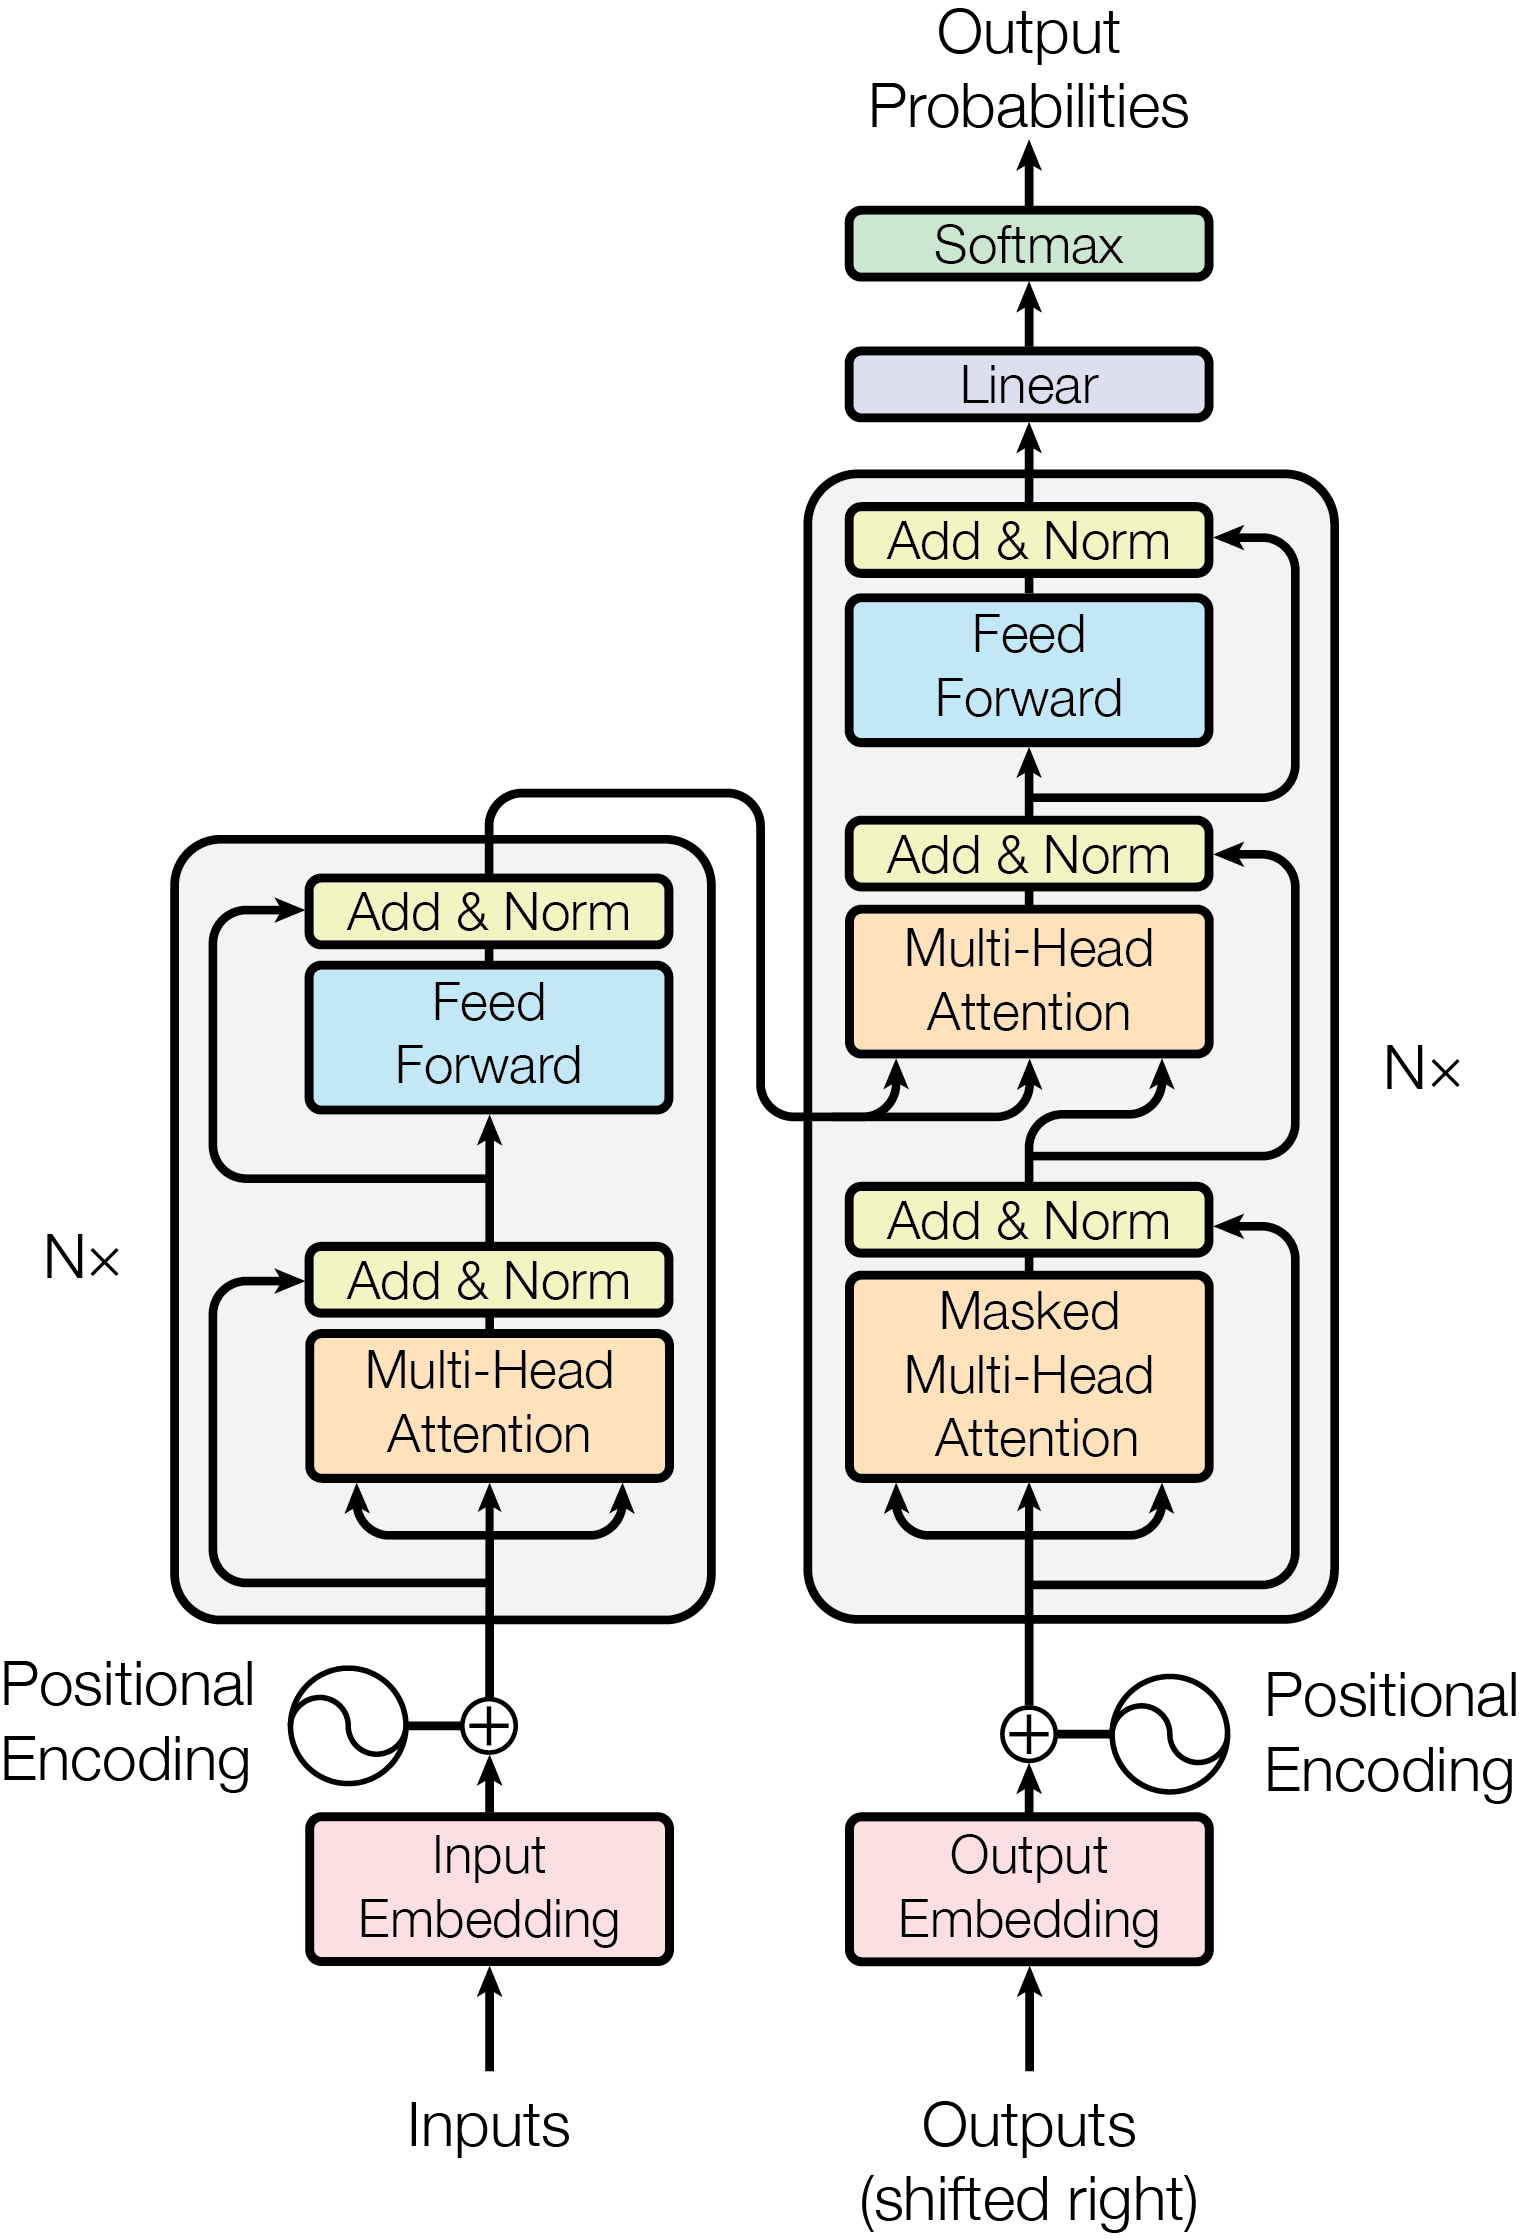
\includegraphics[width=0.4\textwidth]{../extra/transformer.png}
   \caption[Transformer Architecture.]{Transformer Architecture \cite{vaswani_attention_2017}.} 
   \label{fig:transformer-architecture}
\end{figure}

\object{Preprocessing Steps} To prepare the text for the transformer model, several steps are performed before the actual encoding and decoding process begins:

\begin{itemize}
   \item \textbf{Tokenization}. It is a crucial step for transformers and \ac{llms}, where the text is parsed into several units called tokens \cite{naveed_comprehensive_2024,raiaan_review_2024,zhao_survey_2025}. With these, the next step can be performed.
   \item \textbf{Creating Embeddings}. Each token is then converted into a numeric vector representation of the same dimension \cite{vaswani_attention_2017}. By this \cite{raiaan_review_2024}, the token's meaning is mapped in a mathematical space, where comparable phrases are close together, 
   \item \textbf{Positional Encoding}. As mentioned in \cite{vaswani_attention_2017}, positional encoding is added to the input embeddings to provide information about the position of each token in the sequence. This is necessary because transformers do not have a built-in order, unlike \ac{rnns} or \ac{cnns}. 
\end{itemize}

\object{Left: Encoder} The encoder structure is primarily designed for processing and interpreting the input text \cite{wang_history_2024}. It extracts step-by-step features and the result is passed to the decoder \cite{liu_understanding_2024}. Each encoder layer consists of two sublayers: 

\begin{itemize}
    \item \textbf{Orange: Multi-Head Self-Attention Mechanism} \cite{vaswani_attention_2017}. In this layer, every position in the input sequence can attend to all positions in the previous layer of the encoder. By this, told by \cite{patil_review_2024}, the model can capture dependencies between the tokens, regardless of their distance in the input sequence. 
    \item \textbf{Blue: Position-wise \ac{ffn}} \cite{vaswani_attention_2017}. This layer is applied independently to each position in the sequence. By using this layer \cite{liu_understanding_2024}, the encoder can process and extract features from the attention output.
\end{itemize}

\object{Right: Decoder} The decoder instead is responsible for generating the output sequence based on the encoded input. This results in a sequence of generated tokens \cite{raiaan_review_2024}. Each decoder layer is a bit different from the encoder layer structure. It consists of the following three sub-layers:

\begin{itemize}
    \item \textbf{Orange$_1$: Masked Multi-Head Self-Attention Mechanism} \cite{vaswani_attention_2017}. This layer is a modified version of the encoder's self-attention mechanism, but it prevents attending to future positions in the sequence. By this, the model can only use information from the past and current tokens.
    \item \textbf{Orange$_2$: Multi-Head Attention Mechanism} \cite{vaswani_attention_2017}. This layer allows the decoder to attend over the encoder's output, enabling it to incorporate information from the input sequence.
    \item \textbf{Blue: Position-wise \ac{ffn}} \cite{vaswani_attention_2017}. This layer is similar to the one in the encoder, applied independently to each position in the sequence. In the end, the decoder output is passed to a linear layer and a softmax function to finally generate the next-token probabilities.
\end{itemize}

\pagebreak

\object{Resulting Architectures} According to the survey \cite{shao_survey_2024}, the transformer architecture has been split into three main categories, as follows:

\begin{itemize}
   \item \textbf{Encoder-only:} Architectures such as Google BERT \cite{devlin_bert_2019} and its derivates, e.g.\ Huawei ERNIE \cite{zhang_ernie_2019}, Meta RoBERTa \cite{liu_roberta_2019} and Google ALBERT \cite{lan_albert_2020} are solely based on the encoder component. This results a niche for these models being suitable for specific \ac{nlp} tasks focused on comprehension. According to the survey \cite{hou_large_2024}, these models process and encode input into hidden representations to capture word relationships and contextual information. Here, models like BERT observe both the left and right context of the currently focused word.
   
   \item \textbf{Decoder-only}:
   Models like Meta's LLaMA series \cite{touvron_llama_2023}, OpenAI's GPT-1 \cite{radford_improving_2018} to GPT-4 \cite{openai_gpt-4_2024}, and ChatGPT \cite{openai_introducing_2022}, focus on token generation based solely on the preceding tokens. According to the survey \cite{hou_large_2024}, without the reliance on the encoder, decoder-only transformers can be used for diverse generation tasks, such as code generation and code completion.

   \item \textbf{Encoder-Decoder}: Certain architectures such as Google's T5 \cite{raffel_exploring_2023} and their BART model \cite{lewis_bart_2019} integrate both the encoder and decoder components. This leads to hybrid capabilities, combining the understanding of the input and the proper generation of the output. According to \cite{wang_history_2024}, these models are applicable to e.g.\ machine translation, text summarization and question answering. However, the complexity of the dual architecture can lead to demanding training processes and slower inference times.
\end{itemize}

\object{\ac{moe}} As shown in the overview by \cite{naveed_comprehensive_2024}, another notable variant of the transformer architecture is the \ac{moe} \cite{shazeer_outrageously_2017} architecture. In this architecture, multiple experts are integrated. Typically, each \ac{moe} system is a mixture of a \ac{ffn} right after the attention block, and a router mechanism, which decides which token(s) are processed by which expert(s). These are advantageous in terms of computational efficiency while being as powerful as dense models. That means, the size of the model can be increased without increasing the computational cost proportionally, because only a subset of the experts is activated for each input. Prominent examples of \ac{moe} models, obtained from sources besides these above, are xAI Grok-1 \cite{xai_open_2024}, Gemini 1.5 by Google \cite{team_gemini_2024-1}, the DeepSeek models V3 \cite{deepseek-ai_deepseek-v3_2025} and its reasoning variant R1 \cite{deepseek-ai_deepseek-r1_2025}, and the recently released LLaMA 4 family by Meta \cite{meta_ai_llama_2025}.

\vp

\subsection{Framing Bloom's Taxonomy for LLM Applications} \label{sec:blooms-taxonomy}

% \newtodo{We need a bridge from llms to application of bloom with llms}

% Given their advanced capabilities, LLMs enable the automation of the often time-consuming procedure of question generation for educators. The integration of such models into educational settings presents an opportunity to enhance the learning experience, support teachers, and foster the development of educational content. Utilizing LLMs has the potential to assist educators in creating diverse and inclusive materials, thereby freeing up valuable time for teaching and student interaction. However, aligning these automatically generated questions with specific cognitive levels remains a key challenge, requiring careful strategies to guide LLMs effectively

% Given \ac{llms}' capabilities, these enable the automation of the often time-consuming question generation process for educators \cite{vu_chatgpt-based_2024}. The integration of such models into education offers an opportunity to enhance the learning experience, plus support teachers and advance educational content \cite{naveed_comprehensive_2024}. Diverse and inclusive materials can be created with the help of \ac{llms}, thereby freeing up valuable time for both teaching and student interaction \cite{naveed_comprehensive_2024}. However, aligning the \ac{llm}-based questions with specific cognitive levels still remains a key challenge.

Given \ac{llms}' capabilities, these enable the automation of the often time-consuming question generation process for educators \cite{vu_chatgpt-based_2024}. The integration of such models into education offers an opportunity to enhance the learning experience for students and support teachers in advancing educational content \cite{naveed_comprehensive_2024}. 
With the help of \ac{llms}, customized study materials and practice questions can be generated to develop personalized learning for students \cite{al_faraby_analysis_2024,bhowmick_automating_2023,hang_mcqgen_2024}, while freeing up the educators' valuable time for both teaching and student interaction \cite{naveed_comprehensive_2024}.
% sources: 452 part 1 / 453.454 for part 2 
% Diverse and inclusive materials can be created with the help of \ac{llms}, thereby freeing up valuable time for both teaching and student interaction \cite{naveed_comprehensive_2024}. 
% However, aligning the automated questions with specific cognitive levels still remains a key challenge. 

\object{Challenge of Alignment} For automated content creation and personalized learning, the ability to differentiate questions based on certain levels of cognitive complexity is crucial \cite{li_planning_2024,zhuge_twinstar_2025}. However, aligning the automated questions with specific cognitive levels still remains a key challenge. \ac{llms} per se show great potential in \ac{aqg} with respect to different cognitive levels \cite{maity_can_2025,blobstein_angel_2023,duong-trung_bloomllm_2024,scaria_automated_2024,scaria_how_2024}. By using different prompting strategies, as illustrated in the \bfhyperref{sec:performance-enhancements}{Performance Enhancements} and the according \bfhyperref{sec:question-generation-research}{Question Generation Research} section, the models can be guided to generate questions that are aligned with the cognitive levels of Bloom's Taxonomy. Certain approaches can generate questions across all levels of Bloom's Taxonomy \cite{duong-trung_bloomllm_2024,zhuge_twinstar_2025}. However, despite their proficiency at lower levels, \ac{llms} occasionally struggle with adherence at the higher levels \cite{duong-trung_bloomllm_2024,cheng_treequestion_2024,elkins_how_2023}.

\object{Cognitive Hierarchy} In the academic literature, Bloom's Taxonomy \cite{krathwohl_taxonomy_1964} and primarily its revised version \cite{krathwohl_revision_2002} are often discussed in the context of question generation and evaluation with respect to \ac{llms} \cite{zhuge_twinstar_2025,scaria_automated_2024,scaria_how_2024,elkins_how_2023}.
According to \cite{krathwohl_revision_2002}, this taxonomy follows a hierarchical structure where the six main categories are organized by increasing complexity, with each level building upon a less complex predecessor excepting the lowest level. The following figure\footnote{\url{https://citt.ufl.edu/resources/the-learning-process/designing-the-learning-experience/blooms-taxonomy/blooms-taxonomy-graphic-description/}, accessed 04/29/2025} shows the cognitive levels of Bloom's Taxonomy in its revised version.

\begin{figure}[htbp]
   \vspace{-.5em}
   \centering
   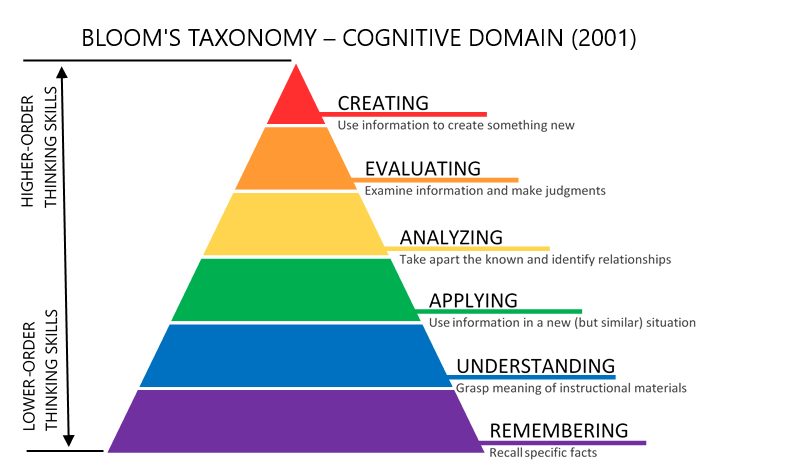
\includegraphics[width=0.65\textwidth]{../extra/Blooms-Taxonomy.png}
   \caption{Hierarchy of Bloom's Revised Taxonomy.}
\end{figure}

The revised taxonomy \cite{krathwohl_revision_2002} is divided into six levels. Each level is associated with a specific cognitive skill, as follows with ascending complexity \tcr{need refinements, bedeutung von wissen??}:
%  representing a different cognitive skill as follows:

\begin{itemize}
   \item \textbf{Remembering:} Formerly known as \enquote{Knowledge}, this level refers to the retrieval of relevant knowledge from long-term memory by focusing on recognition and recall of facts.
   \item \textbf{Understanding:} This level, previously called \enquote{Comprehension}, involves identifying the meaning of instructional messages, such as oral, written and graphic communication.
   \item \textbf{Applying:} This level is about performing or applying a procedure in a given situation.
   \item \textbf{Analyzing:} This involves breaking down material into its components and determining their relationships to one another or to an overall structure or purpose.
   \item \textbf{Evaluating:} This level requires making judgements based on established criteria and standards.
   \item \textbf{Creating:} This is the highest cognitive level and involves assembling or reorganizing elements into a coherent whole.
\end{itemize}

Each of these cognitive levels is associated with a set of action verbs that can be used to formulate learning objectives and assessment questions. A comprehensive list of such verbs, categorized by these cognitive levels, can be found at the University of Arkansas' website\footnote{\url{https://tips.uark.edu/blooms-taxonomy-verb-chart/}, accessed 05/13/2025}. The following table offers a brief overview of the cognitive levels and their corresponding action verbs \tcr{befunde zusammenfassen, wo lücken für mich}

% Du meinst ja oben, dass diese Taxonomy schon genutzt wird, um die Relevanz von LLMs zu untersuchen. Wenn das stimmt, dann würde ich dir empfehlen, hier auch Forschungsbefunde zusammenzufassen. Also was haben die schon untersucht und wo gibt es Forschungslücken, die du jetzt adressieren möchtest

\begin{table}[htbp]
   \centering
   \renewcommand{\arraystretch}{1.6} % Matches row height style from the example table
   \caption{Bloom's Taxonomy Action Verbs.}
   \label{tab:blooms_verbs_columns}
   \begin{tabularx}{\textwidth}{|>{\hsize=1.15\hsize\centering\arraybackslash}X|>{\hsize=1.25\hsize\centering\arraybackslash}X|>{\hsize=0.95\hsize\centering\arraybackslash}X|>{\hsize=0.95\hsize\centering\arraybackslash}X|>{\hsize=0.9\hsize\centering\arraybackslash}X|>{\hsize=0.8\hsize\centering\arraybackslash}X|}
     \hline
     \rowcolor{gray!15}
     \textbf{Remembering} & \textbf{Understanding} & \textbf{Applying} & \textbf{Analyzing} & \textbf{Evaluating} & \textbf{Creating} \\
     \hline
     Define & Clarify & Apply & Analyze & Assess & Assemble \\
     \hline
     Describe & Classify & Calculate & Break down & Conclude & Code \\
     \hline
     Enumerate & Compare & Demonstrate & Detect & Criticize & Compile \\
     \hline
     Identify & Contrast & Determine & Differentiate & Defend & Construct \\
     \hline
     List & Detail & Examine & Distinguish & Evaluate & Create \\
     \hline
     Match & Explain & Illustrate & Examine & Grade & Design \\
     \hline
     Name & Paraphrase & Modify & Investigate & Interpret & Develop \\
     \hline
     Outline & Rewrite & Simulate & Optimize & Judge & Enhance \\
     \hline
     Quote & Summarize & Solve & Relate & Justify & Improve \\
     \hline
     Select & Translate & Use & Separate & Verify & Reorganize \\
     \hline
   \end{tabularx}
 \end{table}

% \object{Application to Question Generation} \ac{llms} show great potential in \ac{aqg} with respect to different cognitive levels \cite{maity_can_2025,blobstein_angel_2023,duong-trung_bloomllm_2024,scaria_automated_2024,scaria_how_2024}. By using different prompting strategies, as illustrated in the \bfhyperref{sec:performance-enhancements}{Performance Enhancements} and the according \bfhyperref{sec:question-generation-research}{Question Generation Research} section, the models can be guided to generate questions that are aligned with the cognitive levels of Bloom's Taxonomy. Certain approaches can generate questions across all levels of Bloom's Taxonomy \cite{duong-trung_bloomllm_2024,zhuge_twinstar_2025}. However, despite their proficiency at lower levels (memory, comprehension), \ac{llms} occasionally struggle with adherence at the higher levels \cite{duong-trung_bloomllm_2024,cheng_treequestion_2024,elkins_how_2023}.

\pagebreak

\subsection{Performance Enhancements}
\label{sec:performance-enhancements}

To address these challenges and to refine the capabilities of \ac{llms} for specific tasks, such as \ac{aqg}, various performance enhancement strategies have been proposed. These techniques aim to improve the quality and relevance of the generated content, as listed in the following:

\object{In-Context Learning} As highlighted by \cite{zhao_survey_2025}, the advent of GPT-3 \cite{brown_language_2020} introduced the concept of in-context learning. OpenAI further delineated this into subcategories such as zero-shot, one-shot, and few-shot learning, depending on how many examples are provided in the prompt.

\object{\ac{cot}} This technique, introduced by \cite{wei_chain--thought_2022}, enhances in-context learning by prompting reasoning steps to elicit the \ac{llms}' step-by-step reasoning \cite{zhao_survey_2025}. Moreover, this method can lead to higher quality questions \cite{scaria_automated_2024}, as depicted in \cite{wei_chain--thought_2022}.
%  [33] in \cite{zhao_survey_2025} --> real source: \cite{wei_chain--thought_2022}

% \object{Being Descriptive} via table 12

\object{Role-based Prompting} This technique involves assigning a specific role or persona to the model while prompting it \cite{zhao_survey_2025} to better fulfill the task instruction. The advantages of the approach are further discussed in the according paper \cite{kong_better_2024} independently of the survey paper.

\object{Self-Refinement} By iteratively refining the \ac{llm}-generated output based on feedback \cite{madaan_self-refine_2023}, the overall process and the corresponding solutions can be improved \cite{zhao_survey_2025}.

% \object{other promptings} from \cite{zhao_survey_2025} what is also to be seen in table 12? 6 new strategies would be nice to mention.

\object{Using Special Marks} Emphasizing important parts of the prompt can be achieved by using special marks like quotation marks or line breaks \cite{zhao_survey_2025} to help the \ac{llm} visually distinguish between different parts of the prompt. 

\object{Positive Constraints} When formulating the prompt, it is often more useful to tell the model what it should do, rather than what it should not do \cite{zhao_survey_2025}. 

\object{Providing Scoring Standards} For tasks which involve scoring a text, it is crucial to provide a detailed description of the scoring standards in the prompt \cite{zhao_survey_2025}. For instance, this clear rubric helps the \ac{llm} to assess the quality of generated questions \cite{scaria_automated_2024}.

% \begin{itemize}
%    \item \textbf{Zero-shot}: To assess the model's ability to generate content without any prior examples or training on a specific task.
%    \item \textbf{Few-shot}: Providing a few examples to guide the model in generating content, compromising between zero-shot and full training.
%    \item \textbf{Role-based prompting}: Providing the model a specific role or persona to adopt, e.g. telling the model to act as an expert in a specific field.
%    \item \textbf{Instructional prompting}: Providing precise instructions to the model to guide its responses.
%    \item \textbf{\ac{cot}}: Dividing the difficult task into smaller and logical steps, so the model can solve the issues step by step. \tcr{was not cited, problem?}
%    \item \textbf{Self-refinement}: Given a problem, building on earlier sub problems, the model refines its own output to solve later subproblems sequentially. \tcr{was not cited, problem?}
% \end{itemize}

% \object{Other Prompting Strategies \cite{zhao_survey_2025}} \tcr{Many interesting strategies to mention}

\object{\ac{rag}} This method \cite{lewis_retrieval-augmented_2020}, as used in approach \cite{hang_mcqgen_2024}, highlights how external knowledge sources can be integrated at \ac{aqg} prompts. For this, querying a comprehensive database is needed to retrieve relevant information that is useful the context of the question. This can be realized via e.g.\ knowledge graphs as domain-specific knowledge, which can be based on course content \cite{yang_heuristic_2024}.

\object{Model Fine-Tuning} A key strategy to adapt general-purpose \ac{llms} to specific tasks by training them on domain-specific data \cite{hou_large_2024}. By this process, models can learn knowledge relevant to a specific context, aber traditional full fine-tuning requires vast amounts of data and computational resources \cite{hou_large_2024}. For instance, \cite{duong-trung_bloomllm_2024} fine-tuned their \ac{aqg} model with more than 1000 questions, which is a relatively small amount of data. % overfitting?

\object{Integration of Contextual Knowledge} Several studies \cite{biancini_multiple-choice_2024,blobstein_angel_2023,wang_towards_2022,bhowmick_automating_2023} have injected topic-related contextual information directly into the prompt to avoid hallucinating and give users control over the source of knowledge \cite{biancini_multiple-choice_2024}.

\vp

\subsection{Evaluation Methodologies}

Evaluation is always necessary to assess the quality of LLMs for the task at hand. According to \cite{doughty_comparative_2024}, evaluating automatically generated learning resources is important because they often lack the deep qualities necessary for their effectiveness.
The methods to evaluate \ac{llms} at e.g.\ \ac{aqg} can be divided into several categories:

\object{$\mathbf{n}$-gram-based Metrics} These metrics follow a reference-based approach, where the generated text is compared to a reference text. The evaluation is based on the overlap of sequences of $n$ words between the generated and reference text \cite{guo_survey_2024}. The most common metrics in this category are:
\begin{itemize}
   \item \textit{\ac{bleu}} \cite{papineni_bleu_2001} evaluates the average $n$-gram precision against a reference text, so how many $n$-grams from the generated text are also present in the reference text \cite{guo_survey_2024}.
   \item \textit{\ac{rouge}}, proposed by \cite{lin_rouge_2004}, calculates recall, which is the ratio of $n$-grams from a ground truth text that are also present in the generated text \cite{guo_survey_2024}.
   \item \textit{\ac{meteor}} \cite{banerjee_meteor_2005} calculates the harmonic mean of precision and recall, so it provides a balanced evaluation \cite{guo_survey_2024}.
\end{itemize}

% -------------------------------------------------------------------------

\object{Diversity-based Metric} The more recent \textit{Distinct-}$n$ \cite{li_diversity-promoting_2016} measures text diversity by calculating the proportion of unique $n$-grams, though it is considered overly simplistic \cite{guo_survey_2024}.

% -------------------------------------------------------------------------

\object{Semantic Similarity} Metrics in this category assess sentence-level comparison, which is vital beyond word-level comparisons \cite{guo_survey_2024}.
\begin{itemize}
   \item \textit{BERTScore} \cite{zhang_bertscore_2020} compares contextual sentence-level embedding vectors from a pre-trained BERT model by calculating cosine similarity between the embeddings of the generated and reference text \cite{guo_survey_2024}.
   \item Manual cosine similarity calculation can also be calculated by comparing embeddings created by an embedding model, as it was done in \cite{li_planning_2024}.
\end{itemize}

\object{Other Metrics} Apart from these categories, diverse other methods and metrics are used to evaluate the generated questions:

\begin{itemize}
   \item For instance, \cite{wang_towards_2022} assessed question quality using \textit{Perplexity} (via GPT-2 \cite{radford_language_2019}), \textit{Diversity} (Distinct-3 score \cite{li_diversity-promoting_2016}), \textit{Toxicity, Grammatical Error,} and the resulting \textit{Acceptability} of a question. \cite{yang_heuristic_2024} also adopted \textit{Perplexity, Diversity,} and \textit{Toxicity}.
   \item Additionally, researchers developing new evaluation metrics often compare their approaches against a range of existing ones. For example, \cite{nguyen_reference-based_2024} benchmarked their proposed metric against \textit{BLEU, ROUGE, BERTScore, QAScore} -- predicting answer extractability from the given context via transformers -- \cite{ji_qascoreunsupervised_2022}, Google's \textit{\ac{bleurt}} -- predicting human judgements of text quality -- \cite{sellam_bleurt_2020}, and the also BERT-based \textit{\ac{rquge}} metric by Meta -- comparing predicted and gold answer spans -- \cite{mohammadshahi_rquge_2023}.
\end{itemize}

% -------------------------------------------------------------------------

\object{Knowledge Graphs} The authors \cite{luo_systematic_2023} presented a framework leveraging knowledge graphs with facts to systematically assess the factual knowledge of LLMs. Frameworks like this can be used to generate questions and their expected answers from given knowledge graph triplets -- such as \texttt{<subject, relation label, object>} -- to evaluate the \ac{llm}'s accuracy.

% -------------------------------------------------------------------------

\object{Human Evaluation} This kind of evaluation is considered necessary to judge about the quality of generated questions \cite{horbach_linguistic_2020}.

\begin{itemize}
   \item While criticizing former used metrics such as \textit{BLEU} and \textit{METEOR} not covering a proper evaluation on question quality, \cite{horbach_linguistic_2020} presented a novel hierarchical evaluation scheme for question generation to guide the human annotators. The scheme often considers binary choices, to induce clear decisions. The following 9 criteria were presented: \textit{Understandable, DomainRelated, Grammatical, Clear, Rephrase, Answerable, InformationNeeded, Central, WouldYouUseIt}. 
   \item Studies such as \cite{steuer_i_2021} and \cite{moore_assessing_2022} adopted this hierarchical scheme and used it for their human question evaluation. For instance, \cite{steuer_i_2021} used it to evaluate their \ac{aqg} system, while \cite{moore_assessing_2022} adopted this scheme to assess the quality of student-generated questions.
   \item Furthermore, the authors in the papers \cite{scaria_how_2024,scaria_automated_2024} used and adapted the evaluation scheme by replacing the criterion \textit{Rephrase} with \textit{Bloom'sLevel}.
   \item  Using \cite{moore_assessing_2022} as a reference, \cite{mi_comparative_2024} proposed another scheme with a maximum of 50 points by covering \textit{Relevance, Clarity, Answerability, Challenging} and \textit{Cognitive Level} as criteria. The latter results in a higher score for questions that are more cognitively demanding, so higher in the Bloom's Taxonomy hierarchy. GPT-4 had most voting agreement with expert ratings in contrast to e.g.\ GPT-3.5 and ERNIE.
   \item Moreover, \cite{moore_automatic_2024} proposed a novel evaluation toolkit for question usability, called SAQUET. Using the 19-item writing flaw rubric by \cite{tarrant_frequency_2006}, they evaluated the \ac{mcqs}. Based on these criteria, the structural and pedagogical value of the questions was assessed, with SAQUET being slightly more strict at rating than the experts.
\end{itemize}

% -------------------------------------------------------------------------

\object{LLM as an evaluator} Another approach involves using \ac{llms} themselves as evaluators. For instance, \cite{nguyen_reference-based_2024} introduced NACo, an \ac{llm}-based metric that employs a \ac{cot} strategy to rank the \textit{Naturalness, Complexity} and \textit{Answerability} of generated questions. In contrast to this, \cite{scaria_how_2024} employed Gemini Pro\footnote{\url{https://blog.google/technology/ai/google-gemini-ai/\#performance}, accessed 05/09/2025} to assess \textit{Question Quality} and \textit{Alignment} with Bloom's Taxonomy, revealing discrepancies compared to human evaluators. It is noteworthy that the abilities of \ac{llms} are rapidly evolving, and results from former models, e.g.\ Gemini Pro, might differ with versions nowadays. 

Other research has also explored using \ac{llms} for tasks like classifying question quality, evaluating answerability, or performing other evaluations based on predefined criteria \cite{moore_assessing_2022,scaria_how_2024,blobstein_angel_2023}. The use of \ac{llms} for evaluation is a promising direction, especially when coupled with human evaluation. Comparing the agreement between the \ac{llm} and the experts can enhance the reliability of the evaluation process.

\vp

\section{Related Work} \label{sec:related-work}

This section explores current research in \ac{llms} and their application to \ac{aqg}, with sections to detail the literature review process and highlight significant contributions in the field.

% \newtodo{Discuss other work in the field aiming this related research problem.}
% \newtodo{Show how my research builds on them, where used for inspiration, and e.g. how approaches may be combined.}
% \newtodo{Mention papers, explain why good or bad, also in comparison with my approach.}
% \newtodo{Try to categorize and group the related work by these, show (dis)advantages using one example.}

\object{Literature Review} To find the fundamental principles and state-of-the-art of the research problem, a literature review was conducted. It was performed in the following way: First, several searches were done with respect to \ac{llms} in common, question generation, particularily focusing on Bloom's Taxonomy, and lastly evaluation methods for both categories. Google Scholar and Elicit were used to find relevant papers. Several search terms were coupled in Google Scholar, such as \textit{LLM, Large Language Model, architecture, question generation, automatic question generation, Bloom's Taxonomy, evaluation, assessment, alignment}. Elicit is a search engine that is designed to help researchers find relevant papers based on writing a specific prompt, instead of a query of keywords.

\object{Review Steps} The review steps were as follows: 
\begin{itemize}
    \item First, the papers were downloaded and stored in Zotero. Then, duplicates were filtered out.
    \item The remaining papers were \textbf{included} or excluded by using the TACID method. Papers were included if they are recent (published from 2021 on) and dealing with LLMs or automated question generation or evaluation methods. If the paper was a preprint instead of a peer-reviewed paper, it needed a comparatively high relevance to be included ($\approx 10$ citations). If a publication was present in a workshop, it needed citations to be included.
    \item Papers were \textbf{excluded} if they were not written in English, not open access, or the journal is predatory\footnote{Journals noted on \url{https://beallslist.net/}, accessed 04/30/2025}. If the focus is explicitly on \ac{slms} or multimodal models, or other domains besides the desired ones, the paper was excluded. 
    \item After the process, the remaining papers were filtered by a deeper analysis of the papers.
    \item In the end, diverse cited and subsequently found papers blog posts by e.g.\ Google were added to the thesis to improve the information space.
\end{itemize}

\subsection{Current LLMs Research}

\hspace{1.5em}\object{Review Challenges at \ac{llms}} Finding the current state-of-the-art of \ac{llms} with the explained review method did not yield recent results, even if papers such as surveys were published in 2024 or 2025. The reason for this is that the field of \ac{llms} is moving so fast, that the review papers become outdated. So, the trend of the models and their releases were followed manually, as captured in Table \bfref{tab:llm_releases}. It shows the most important releases of \ac{llms} in the past years since ChatGPT \cite{openai_introducing_2022}. The table is not complete, but it shows well-known models and their architecture, including \textit{reasoning} capabilities, if these are known to the public. Reasoning means, in the OpenAI o1 system card \cite{openai_openai_2024-1} for instance, the model thinks in a manner of \ac{cot} before responding to the user. The table is sorted by the release date of the models to obtain a timeline and a way to interpret the development of the models.

\pagebreak

\object{Major LLM Developers and Models} The following list details prominent developers in the \ac{llm} space and provides an overview of their key model releases and architectural trends.
\begin{itemize}
    \item \textbf{OpenAI:} With the initial release of ChatGPT \cite{openai_introducing_2022}, which firstly utilized the GPT-3.5 architecture, OpenAI has limited the disclosure of architectural details for its subsequent models. The GPT-4 model \cite{openai_gpt-4_2024} was followed by GPT-4o \cite{openai_gpt-4o_2024}, which outperformed GPT-4. The \enquote{GPT} nomenclature indicates a continuation of the decoder-only transformer architecture, a characteristic of known models up to GPT-3 \cite{brown_language_2020}. OpenAI's current state-of-the-art models emphasize reasoning capabilities, as seen in the o1-mini \cite{openai_openai_2024}, o1 \cite{openai_openai_2024-1}, o3-mini \cite{openai_openai_2025}, and the subsequent o3 and o4-mini \cite{openai_openai_2025-1} releases.

    \item \textbf{Meta:} Meta has provided some architectural insights for its LLaMA series. The first generation \cite{touvron_llama_2023} was based on a modified transformer architecture. LLaMA 2 \cite{touvron_llama_2023-1}, up to the LLaMA 3.3 iteration adopted a decoder-only transformer\footnote{\url{https://github.com/meta-llama/llama-models/blob/main/models/llama3_3/MODEL_CARD.md}, accessed 05/09/2025. Note that auto-regressive means decoder-only}. With LLaMA 4 \cite{meta_ai_llama_2025}, Meta also transitioned to \ac{moe} models, with a maximum of 2 trillion parameters on its third model.

    \item \textbf{Google:} Google's Bard, launched in February 2023, was initially based on the LaMDA architecture \cite{pichai_important_2023,thoppilan_lamda_2022}, making it a decoder-only model. Subsequent fine-tuning led to the Gemini series \cite{team_gemini_2024}, which also started as decoder-only. Gemini 1.5 marked a shift to an \ac{moe} architecture, though still described as decoder-based \cite{team_gemini_2024-1}. Beginning with Gemini 2.0 \cite{pichai_introducing_2024}, Google stopped publishing detailed architectural information. Gemini 2.5 \cite{kavukcuoglu_gemini_2025} further advanced their offerings by fully integrating reasoning capabilities, aligning with current state-of-the-art trends.

    \item \textbf{Anthropic:} Anthropic has maintained the policy of not disclosing detailed architectural information for its Claude series. This applies from the initial Claude 1 \cite{anthropic_introducing_2023} and Claude 2 \cite{anthropic_claude_2023} models, through the Claude 3 family \cite{anthropic_introducing_2024-1}, Claude 3.5 Sonnet \cite{anthropic_introducing_2024}, and up to Claude 3.7 Sonnet \cite{anthropic_claude_2025}. The latter also incorporated reasoning capabilities, making it competitive with other currently leading models.

    \item \textbf{xAI:} xAI initially disclosed that its Grok-1 model utilized an \ac{moe} architecture \cite{xai_open_2024}. However, for subsequent releases, Grok-2 \cite{xai_grok-2_2024} and Grok-3 \cite{xai_grok_2025}, architectural details were not provided, though Grok-3 is a competitive state-of-the-art model with reasoning.

    \item \textbf{DeepSeek AI:} DeepSeek AI offers open-source models, with DeepSeek V3 \cite{deepseek-ai_deepseek-v3_2025} as a popular \ac{moe} model. One month later, DeepSeek R1 \cite{deepseek-ai_deepseek-r1_2025} followed, reportedly using the same architecture but with added reasoning capabilities.

    \item \textbf{Alibaba:} The Alibaba Group has also contributed to the field with models like Qwen 2.5-Max \cite{team_qwen25-max_2025}, an \ac{moe} model. The more recent QwQ-Max \cite{team_thinkthink_2025} builds upon this architecture, incorporating reasoning to compete at the state-of-the-art.
\end{itemize}

\pagebreak

Visible in Table \bfref{tab:llm_releases}, the current state-of-the-art for the given table began from o1 and o3-mini in December 2024 plus the release of DeepSeek V3. January 2025, DeepSeek R1 and Alibaba's Qwen 2.5-Max model without reasoning capabilities were released. February 2025 brought xAI's Grok-3, Anthropic's Claude 3.7 Sonnet and Alibaba's QwQ-Max. In March 2025, the state-of-the-art was reached by a major upgrade in Google Gemini, with the release of Gemini 2.5. Finally, April 2025 featured the LLaMA 4 family by Meta and OpenAI's o3 and o4-mini models. Based on this information pool, the models for the \ac{aqg} evaluation were selected, as to be seen in Section \bfref{sec:experiment-design}. 

\object{Key \ac{llm} Development Trends} As illustrated in Table \bfref{tab:llm_releases}, a discernible trend is the decreasing transparency from developers regarding architectural designs of their \ac{llms}. While some models are known to be transformer-based (e.g.\ decoder-only) or employ an \ac{moe} architecture, and reasoning capabilities are often highlighted, many other details remain undisclosed due to the competitive nature of the field. It is also worth noting that there is a trend towards models with a higher number of parameters, a prevalence of decoder-only architectures from ChatGPT on, and an increasing adoption of \ac{moe} designs, a trend possibly popularized by GPT-4. Although the technical report for GPT-4 \cite{openai_gpt-4_2024} lacks architectural specifications, it is rumored to be an \ac{moe} model\footnote{\url{https://medium.com/@seanbetts/peering-inside-gpt-4-understanding-its-mixture-of-experts-moe-architecture-2a42eb8bdcb3}, accessed 05/09/2025}. Furthermore, a significant trend is the continuous integration of reasoning capabilities into \ac{llms}, with the most recent models being competitive in this area.

\subsection{Question Generation Research}
\label{sec:question-generation-research}

\ac{llms} enable the automation of the time-consuming and demanding procedure of question generation \cite{vu_chatgpt-based_2024}. It has been communicated by the authors \cite{naveed_comprehensive_2024}, that the integration of such models into educational settings offer an opportunity to improve the learning experience, support teachers and encourage the development of educational content. The utilization of \ac{llms} has the potential to assist educators in the creation of diverse and inclusive materials with respect to education. This results in freeing up time for educators to focus on teaching and interacting with students.

\object{Focusing solely on Prompt Engineering} Several studies have investigated the capability of \ac{llms} to generate educational questions aligned with cognitive levels, primarily by refining and optimizing the prompts given to the models. These approaches aim to guide \ac{llms} towards producing questions that meet specific educational objectives without any modification of the underlying model architecture.
\begin{itemize}
    \item \cite{blobstein_angel_2023} developed Angel, a tool that utilizes GPT-3.5 for generating questions at varying cognitive levels based on Bloom's Taxonomy. The system employs instructional prompts with a few-shot learning approach and textbook content to produce questions categorized by difficulty (easy, medium, hard). The evaluation of the generated questions and their answers was conducted using GPT-3.5 again as an evaluator with a \ac{cot} strategy, focusing on metrics such as \textit{Clarity, Relatedness, Importance,} and \textit{Answerability}. Human evaluation was also performed.
    \item \cite{scaria_how_2024} assessed the capability of \ac{llms}, including GPT-3.5 and GPT-4, to generate high-quality questions across different cognitive levels using zero-shot prompting. The CEFR level was also specified in the prompts. Two annotators evaluated the generated questions based on categories adapted from \cite{horbach_linguistic_2020}, where the \textit{Rephrase} category was modified to \textit{Bloom'sLevel} to assess adherence to the targeted cognitive level. The Inter-annotator agreement was measured using Cohen's Kappa \cite{cohen_coefficient_1960}. Their findings suggest that \ac{llms} can produce relevant and high-quality questions at diverse cognitive levels, indicating their utility for scalable educational content generation, with GPT-4 and GPT-3.5 being notably effective.
    \item \cite{elkins_how_2023} investigated steering question generation with InstructGPT \cite{ouyang_training_2022} by employing a combination of Bloom's Taxonomy and a difficulty-level taxonomy \cite{perez_automatic_2012}, including \textit{Beginner, Intermediate, Advanced}. The generated questions were assessed by 19 annotators (11 from biology and 8 from machine learning) on criteria including relevance, grammar, adherence to the taxonomy, answerability, and usefulness. Inter-annotator agreement was determined using Cohen's Kappa. The study concluded that five-shot prompting was more effective than zero-shot prompting for this task.
    \item \cite{maity_can_2025} explored the potential of \ac{llms} for \ac{aqg}, with a focus on Bloom's revised Taxonomy. Using the same evaluation metrics as \cite{elkins_how_2023}, the study compared simple zero-shot prompting against eight-shot prompting. 16 school teachers evaluated the generated questions, finding that eight-shot prompting improved the quality of educational questions. GPT-4-turbo was identified as the best performing model under both prompting conditions. 
    \item \cite{al_faraby_analysis_2024} investigated the use of \ac{llms} for educational question generation with ChatGPT vs. LLaMA2-13B. The study focused on textbook-based questions and different prompting strategies: zero-shot, enhanced zero-shot, few-shot, and few-shot with \ac{cot}, with each version tested via 6 variations. Human evaluators (experts and crowdsourcing) were employed, revealing that experts preferred human-generated questions from textbooks, while crowdsourced evaluators illustrated comparable preferences for both human- and \ac{llm}-generated questions. The enhanced zero-shot approach outperformed the other methods. The evaluation included metrics such as \textit{Clarity, Alignment with Learning Objectives} (obtained from the textbooks' sections), \textit{Simulation to critical Thinking, Usefulness, Difficulty Level}, and \textit{Resemblance to Human-generated Questions}. Also, the inter-rater agreement was measured using Cohen's Kappa.
    \vspace{9em}\pagebreak
    \item \cite{vu_chatgpt-based_2024} aimed to support educators in generating question banks in higher education using ChatGPT. Drawing inspiration from \cite{cavojsky_exploring_2023}, the authors established several prompt patterns for each question type (Multiple-Choice, True-False, Calculative Exercise). For instance, a combined prompt called RTCEF was used, which included the \ac{llm}'s role, the desired task, context, an example, and the output format. While noting the potential for supporting educators, the study highlighted issues with calculative exercises. These questions were often filtered out due to insufficient data, relying on the probability of word appearance rather than logical factors for generation. Their evaluation conducted a blind test where lecturers were best able to differentiate between human- and \ac{llm}-generated questions, while students' groups showed less accuracy.
\end{itemize}

\object{Focusing solely on \ac{llm} Fine-Tuning} Another avenue of research involves fine-tuning pre-trained \ac{llms} on domain-specific or task-specific data to enhance their question generation capabilities. This approach aims to adapt the models to better understand educational contexts and produce more relevant and accurate questions.
\begin{itemize}
    \item \cite{duong-trung_bloomllm_2024} introduced BloomLLM, a fine-tuned GPT-3.5-turbo model, which was developed to generate educational questions with respect to Bloom's Taxonomy via descriptive zero-shot prompting. The fine-tuning was based on manually annotated questions considering the cognitive levels of Bloom's Taxonomy. 46 master's students were asked to tell which questions were preferred, and the results show that BloomLLM's questions have a higher relevance across all levels of Bloom's Taxonomy in contrast to the successor GPT-4.
    \item \cite{lamsiyah_fine-tuning_2024} propose RLLM-EduQG, a system that consists of a fine-tuned Google FLAN-T5 model for \ac{aqg}. From text passages, the model generates questions and answers. The authors employed two reward functions to guide the model's learning process: the BLEU metric and a semantic reward function. RLLM-EduQG was evaluated using several simple metrics, including \textit{BLEU, F1, ROUGE, Perplexity,} and \textit{Diversity}, indicating a high predictive and linguistic quality.
\end{itemize}

\object{Integrated Systems\,/\,Hybrid Architectures} Researchers have also developed more complex systems that integrate \ac{llms} with other components or employ multiple \ac{llms} in a coordinated fashion. These hybrid architectures often aim to leverage the strengths of different techniques to achieve more robust and diverse question generation.
\begin{itemize}
    \item \cite{cheng_treequestion_2024} proposed TreeQuestion, a system utilizing GPT-3.5-turbo for generating \ac{mcqs}. Their approach follows an \enquote{Explore-Validate-Generate} pattern: initially, an \ac{llm} generates knowledge graphs in a zero-shot setting to explore concepts, which educators can then validate. Subsequently, TreeQuestion generates questions aiming for alignment with Bloom's Taxonomy levels. A software interface allows educators to select Bloom's levels and set question difficulty. Evaluation by 10 teachers and 96 students indicated that the generated \ac{mcqs} were comparable in overall quality to human-generated open-ended questions. The study also discussed limitations, such as generating questions requiring complex cognitive processes like intricate reasoning. The system used Bloom-based, zero-shot prompts and focused on time-saving for educators.
    \item \cite{doughty_comparative_2024} conducted a comparative study of \ac{mcqs} generated by GPT-4 versus those created by humans. The authors developed a system that generates \ac{mcqs} from course context, primarily focusing on learning objectives. These objectives were aligned with Bloom's Taxonomy levels using a fine-tuned BERT classifier. Human evaluation indicated that GPT-4 produced \ac{mcqs} comparable to human-generated ones in terms of clarity, distractor quality, and learning objective coverage. The system utilized descriptive and instructional few-shot prompts that also explained the Bloom's levels, without providing any context for the \ac{llm}-based questions.
    \item \cite{zhuge_twinstar_2025} developed TwinStar, a novel system employing a dual-\ac{llm} engine for educational question generation. The system utilizes two-shot prompting based on multiple rounds, recognizing that advanced \ac{llms} like GPT-4 struggle with precise adherence to Bloom's Taxonomy levels. Therefore, the authors fine-tuned ChatGLM2-6B \cite{glm_chatglm_2024} and LLaMA2-13B \cite{touvron_llama_2023-1}, with LLaMA2-13B demonstrating superior performance. TwinStar operates through an iterative process involving two engines: one for question generation and another for evaluation. The evaluation model was fine-tuned on 1000 questions to better recognize Bloom level features. If a generated question aligns with the target Bloom's level and passes a redundancy check, it is accepted. Otherwise, the generation model refines the question based on feedback from the evaluation model to achieve the desired cognitive level. Experiments demonstrated TwinStar's superior performance in Bloom's Taxonomy adherence compared to \ac{llms} such as Bard, Claude 3, and GPT-4.
    \item \cite{yang_heuristic_2024} addressed hallucination, which is unacceptable in education. Moreover, the authors proposed a system based on \ac{rag}, leveraging a knowledge graph constructed from course content to supply domain-specific knowledge. For knowledge retrieval, a fine-tuned BERT model was employed, and GLM-4 \cite{glm_chatglm_2024} was the utilized \ac{llm} for question generation. The Prompts included task descriptions, reasoning examples, knowledge paths, and the target Bloom cognitive levels. Ultimately, the evaluation focuses on aspects like \textit{Perplexity, Diversity} and human evaluation with 20 students based on a certain statement list of 12 items.
    \item \cite{hang_mcqgen_2024} presented MCQGen, a system that generates \ac{mcqs} for personalized learning by using GPT-4. They employed \ac{rag} and advanced prompting techniques, drawing on an external knowledge base. The approach leveraged the advanced semantic understanding and summarization capabilities of GPT-4. Both human- and \ac{llm}-based evaluators were used to assess the generated questions to provide a comprehensive assessment. Mixed outcomes were observed between e.g.\ LLaMA2 and GPT-3.5 versus human lecturers. While utilizing \ac{cot} prompting with self-refinement, the evaluation focused on \textit{Grammar, Answerability, Diversity, Complexity,} and \textit{Relevance}. Diversity and answerability lacked in both evaluation methods, suggesting that prompt optimization and expanding the knowledge base could address these limitations. 
\end{itemize}

\vspace{3em}\pagebreak

\object{Research Gaps addressed by this Thesis} ...

\newtodo{Maybe the texts above need a little refinement, so that the gaps are more visible.}

\newtodo{Create proper research gaps text, what do i want to address with my thesis?}

\begin{itemize}
    \item outdated models or small language models used, even in current papers
    \item uprising reasoning/thinking capabilities were not considered
    \item "A significant research gap exists regarding the creation of
cognitively challenging questions, particularly the effective implementation and scoring of questions
aligned with higher levels of Bloom's Taxonomy. While LLMs such as ChatGPT [Ope22] are good
at generating questions for lower cognitive levels, they have limitations at the higher levels, often
generating oversimplified or unrealistic questions [DWK24; Elk+23; SDS24]"
    \item what else?
\end{itemize}
\vp

\section{Experimental Design}
\label{sec:experiment-design}

Two experiments were conducted to evaluate the performance of a selected set of \ac{llms} in generating questions. The first experiment primarily focused on the \textbf{RQ1}, which aimed to assess the content fidelity of the generated questions according to the \ac{llms} and the diverse source materials. The second experiment was designed to answer \textbf{RQ2}, which focused on analyzing the relationships between the \ac{llms}, given questions formats and given levels of Bloom's revised Taxonomy \cite{krathwohl_revision_2002}.

\begin{figure}[htbp]
    \centering
    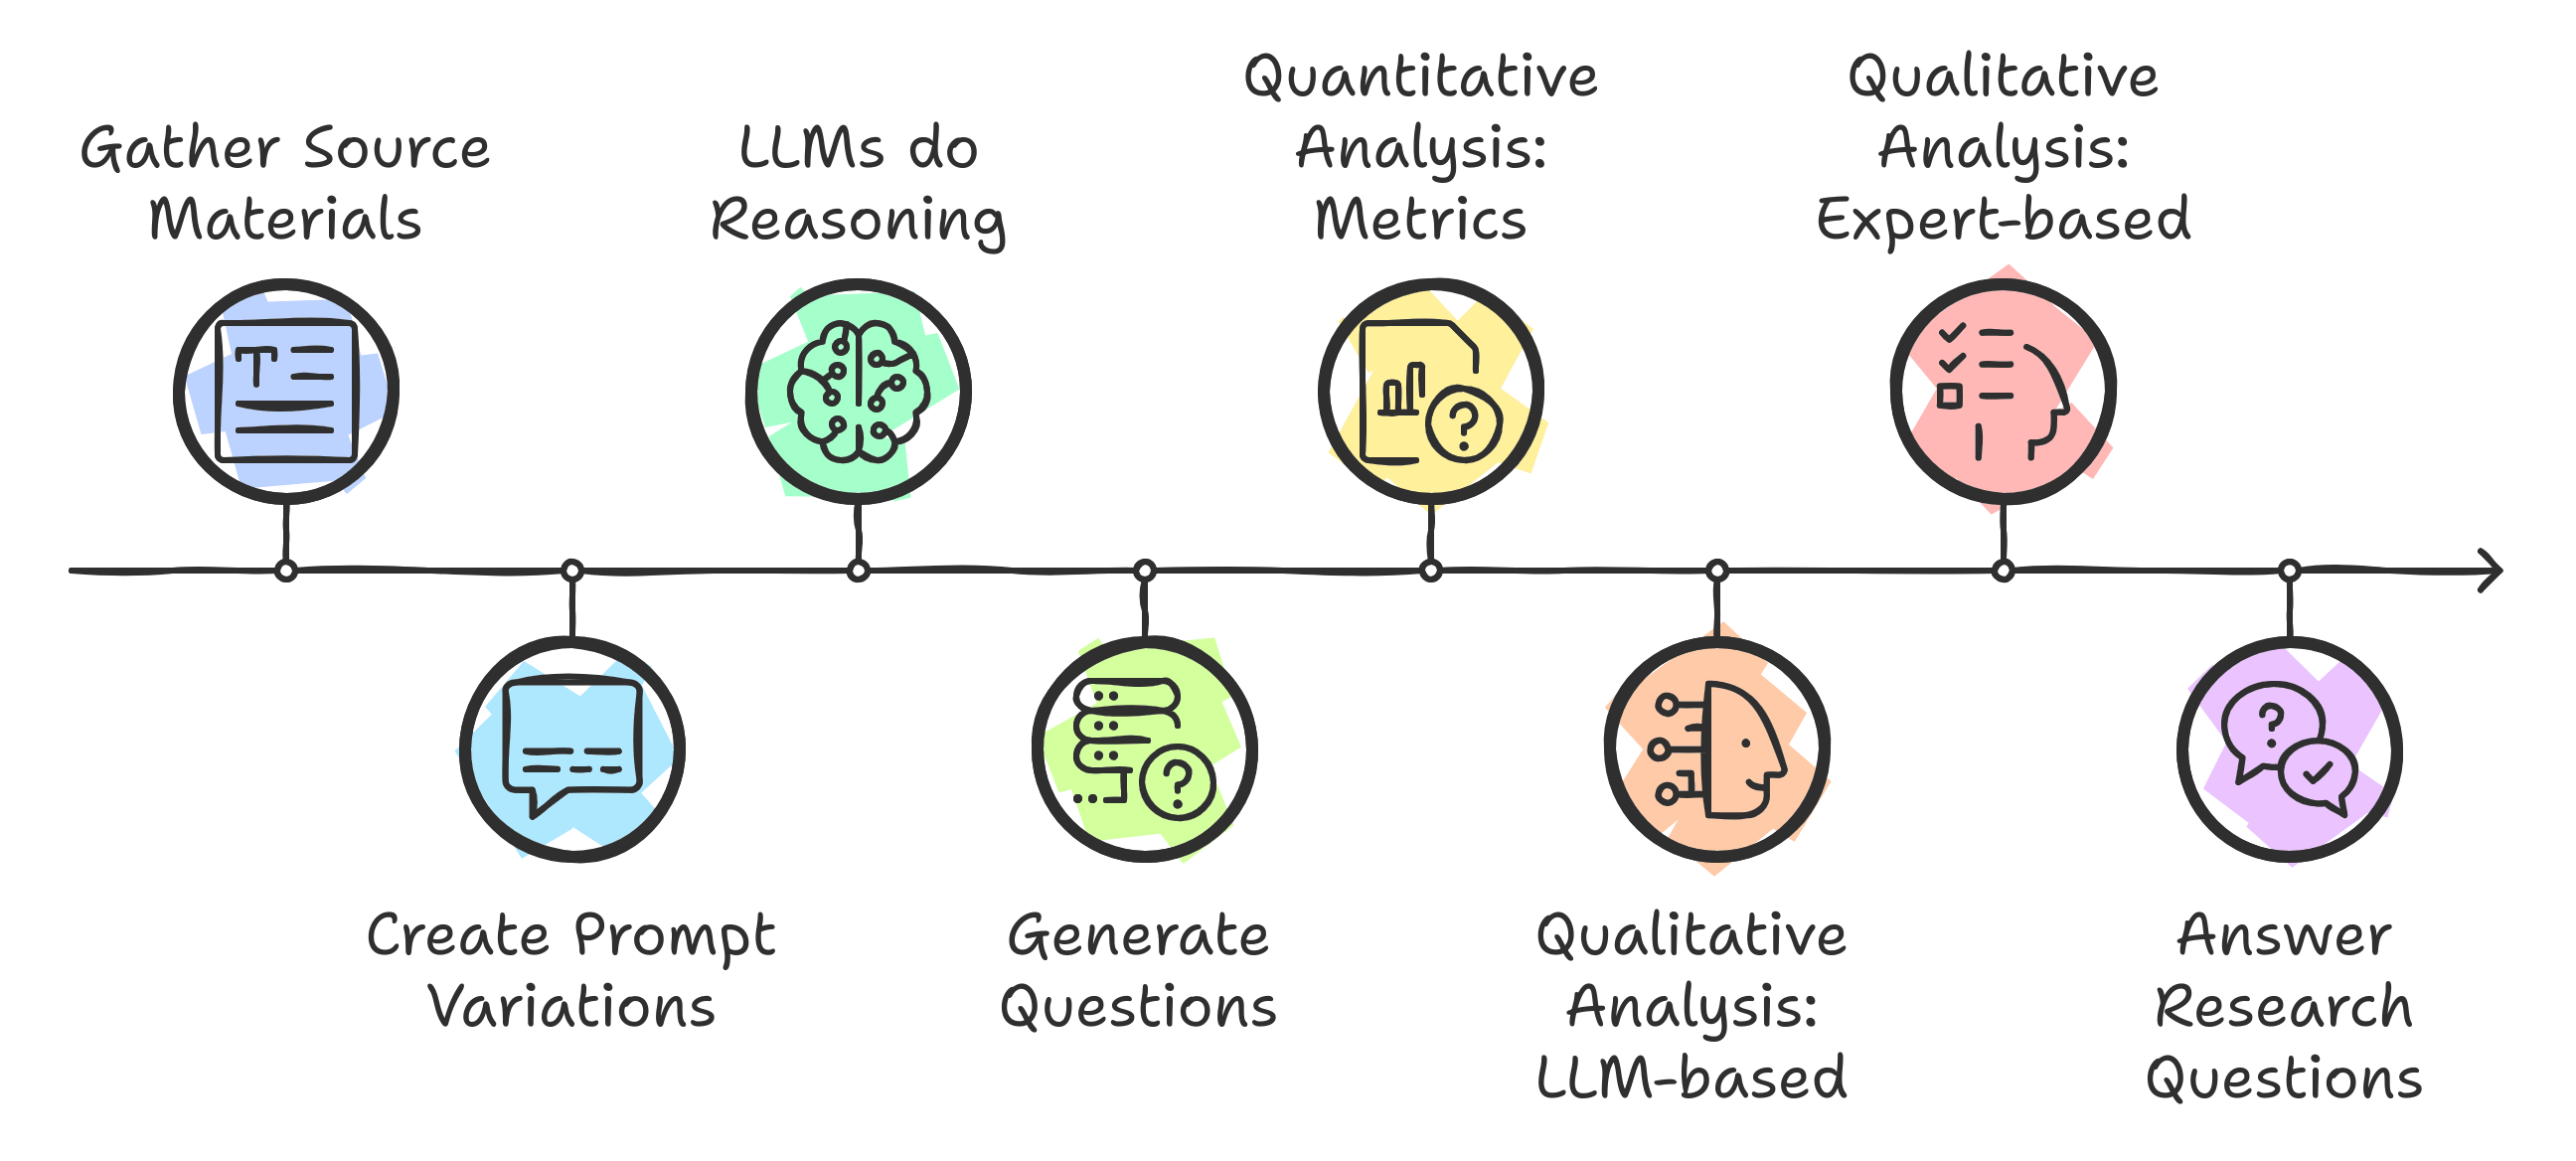
\includegraphics[width=\textwidth]{../extra/approach.png}
    \caption[Experimental Pipeline.]{Experimental Pipeline\footnotemark.}
    \label{fig:experiment-overview}
\end{figure}
\footnotetext{created with \url{https://www.napkin.ai/}, accessed 05/24/2025}
\vspace{-1em}
    
\subsection{Selection of Resources}
\label{sec:selection-resources}

To ensure the experiments were well-structured and relevant, a variety of resources were selected. This covers the source materials and the \ac{llms} used in the experiments for \ac{aqg}.

\object{Selection of Source Materials}
Focusing on the subject of the ISO-OSI model, the following materials, illustrated \bfhyperref{sec:source_materials}{here}, were diversely used to generate the experiments' questions:

\begin{itemize}
    \item \bfhyperref{sec:script-common}{Lecture Slides} \textbf{(extracted Part)}: Dealing with reference architectures, the ISO-OSI model is presented in detail. The slides are in German and were used for \ac{aqg} for the first experiment.
    \item \bfhyperref{sec:transcript}{Transcript} \textbf{(Lecture's Video Part)}: The transcript of the extracted slides is in German and was also used to generate questions for the first experiment.
    \item \bfhyperref{sec:tanenbaum}{Book's Excerpt} \textbf{(from \enquote{Computer Networks})} \cite{tanenbaum_computer_2013}: This book is in English and was used to generate questions for both experiments, with a detailed description of the ISO-OSI model, including all seven layers.
\end{itemize}

To properly challenge the \ac{llms} in their multilingual capabilities, each source material was kept in its original language: German for the lecture slides and its transcript, the book excerpt in English.

\pagebreak

\object{Selection of \ac{llms}} A total of four \ac{llms} were selected for both experiments, which belong to the current state-of-the-art in the field of \ac{llms} and are publicly available to certain degrees, and incorporate reasoning capabilities. The selected models are:
Anthropic Claude 3.7 Sonnet \cite{anthropic_claude_2025},
    DeepSeek R1 \cite{deepseek-ai_deepseek-r1_2025},
    Google Gemini 2.5 Flash \cite{kavukcuoglu_gemini_2025}, and
    OpenAI o3 \cite{openai_openai_2025-1}.

\vspace{1em}

o3 and Claude 3.7 Sonnet were accessed through their Python APIs\footnote{\label{fn:openai-api}\url{https://github.com/openai/openai-python}, accessed 05/09/2025}\footnote{\label{fn:anthropic-api}\url{https://github.com/anthropics/anthropic-sdk-python}, accessed 05/09/2025}, incurring costs per usage. This access method was necessary as the chosen models were not available to the required extent through other means. In contrast, Gemini 2.5 Flash was utilized via Google's Python API\footnote{\label{fn:google-api}\url{https://github.com/googleapis/python-genai}, accessed 05/09/2025}, which offers a free usage tier. To manage costs while maintaining a robust set of \ac{llms}, DeepSeek R1, a comparatively less expensive yet highly capable \ac{llm}, was accessed free of charge via its website\footnote{\label{fn:deepseek}\url{https://chat.deepseek.com/}, accessed 05/09/2025}.

\subsection{Methodological Approach}
\label{sec:methodological-approach}

The method employed for the two experiments is outlined here. It details the specific procedures for generating questions, including the variations in source materials, \ac{llm} prompting strategies, and the targeted number of questions for each experimental condition.

% \object{Experiment 1a: Content Fidelity} The presented 4 source materials were used to generate questions. The 4 state-of-the-art \ac{llms} were used, each model was prompted with the 4 input types each via a common prompt and a complex prompt. 
% \newtodo{Think about splitting the inputs into 7 groups, related to the 7 ISO-OSI layers.}
% This would result a final set of questions: 4 materials / or 28 if thinking about the 7 layers, 4 \ac{llms}, 5 questions for each prompt, 2 prompts, $4\cdot 4\cdot 5\cdot 2=160$

\object{Experiment 1a: Content Fidelity} For the first experiment, questions were generated using the three selected source materials to compare the questions' quality. All four state-of-the-art \ac{llms} were employed. Each model was prompted using both a simple and a complex prompt. To prevent context spillover and ensure focused questioning, one question was generated per prompt for each of the seven layers of the ISO-OSI model, with the context for each layer being introduced in each distinct run. This methodology resulted in a total of \begin{align}4 \text{ \ac{llms}} \times 3 \text{ input sources} \times 7 \text{ layers} \times 1 \sfrac{\text{ question}}{\text{prompt}} \times 2 \text{ prompts} = 168 \text{ questions.}\end{align}

% \object{Experiment 1b: Error Propagation} A second run is to be done. The same experimental setup as in Experiment 1a was used, but the source materials were manipulated. I have to choose a certain layer of the ISO-OSI model and manipulate the source materials for this layer. So there is 1 layer only, and 3 source materials (the system knowledge only is not used). 4 \ac{llms} used again, 5 questions per prompt, 1 prompt (the complex and better one). This results in a final set of questions: $1\cdot 3\cdot 4\cdot 5\cdot 1=60$.

\object{Experiment 1b: Error Propagation} A subsequent run focused on error propagation. The four \ac{llms} were again utilized with both simple and complex prompts. For this experiment, a single input source, specifically the lecture script -- chosen for its concise and precise contextual information -- was used. Each of the seven layers of the ISO-OSI model within this source material was intentionally manipulated to introduce errors, as to be seen \bfhyperref{sec:script-manipulated}{here}. Seven questions were generated per prompt, one for each manipulated layer and run. This resulted in a total of \begin{align}4 \text{ \ac{llms}} \times 1 \text{ input source} \times 7 \text{ layers} \times 1 \sfrac{\text{ question}}{\text{prompt}} \times 2 \text{ prompts} = 56 \text{ questions.}\end{align}

\pagebreak

\object{Experiment 2: Question Formats and Bloom's Taxonomy} The second experiment focused on the generation of varied question formats and their alignment with Bloom's revised Taxonomy. Contextual information for this experiment was derived from a single, pre-selected layer of the ISO-OSI model, utilizing the detailed content from \bfhyperref{lst:tanenbaum_layer2}{Layer 2} within the excerpt from \cite{tanenbaum_computer_2013}. The four selected \ac{llms} were employed in three distinct runs, each designed to explore different prompting parameters related to question type and cognitive complexity:

\begin{enumerate}
    \item \textit{Question Type Specification}: Prompts specified only the desired question types (Multiple-Choice and Open-Ended). For the chosen layer, each \ac{llm} was tasked six times to generate a question without mentioning a certain Bloom level for each of the two question types, resulting in \begin{align}4 \text{ \ac{llms}} \times 2 \text{ question types} \times 1 \sfrac{\text{ question}}{\text{run}}\times 6 \text{ runs} = 48 \text{ questions.}\end{align}
    \item \textit{Cognitive Level Specification}: Prompts specified only the target cognitive levels according to Bloom's Taxonomy. For the chosen layer, each \ac{llm} generated one question for six runs to get a question for each of the Bloom levels. In total, these are  \begin{align}4 \text{ \ac{llms}} \times 1 \sfrac{\text{ question}}{\text{level}} \times 6 \text{ Bloom levels} = 24 \text{ questions.}\end{align}
    \item \textit{Combined Specification}: Prompts specified both the question types (Multiple-Choice and Open-Ended) and the cognitive levels. Similar to the first run, this resulted in \begin{align}4 \text{ \ac{llms}} \times 2 \text{ question types} \times 1 \sfrac{\text{ question}}{\text{level}} \times 6 \text{ Bloom levels} = 48 \text{ questions.}\end{align}
\end{enumerate}

\object{Data Collection} The data was primarily collected using the \ac{llms} via their APIs, excepting DeepSeek being prompted on the website. The other 3 models were prompted automatically via Python to generate questions based on the given source materials. The generated questions were stored in a directory structure, particularly based on the experiment, the \ac{llm} and the source material. The question files for each prompt were stored in distinct \textit{.txt} files.

\object{Evaluation Plan} The evaluation of the generated questions will be conducted in two phases, corresponding to the two main experiments. Each phase employs a multi-modal assessment combining automated metrics, LLM-based evaluation, and expert human annotation to ensure comprehensive quality assessment.
\begin{itemize}
    \item \textbf{Experiment 1 (Content Fidelity and Error Propagation):}
    \begin{itemize}
        \item \textit{Quantitative Analysis:} In this stage, the \textit{Semantic Similarity} between generated questions and source materials will be assessed using cosine similarity on generated text embedding vectors. This can be done since a sentence transformer is used, which offer comparable sentence embeddings \cite{reimers_sentence-bert_2019}. Metrics such as \textit{\ac{bleurt}} and \textit{\ac{rquge}} were not employed since, on the one hand, the structure of the source material and the question differ too much, and on the other hand, gold standard answers are not available for comparison.

        \pagebreak
        
               
        Moreover, other metrics such as Perplexity are unsuitable for this task, as \enquote{the output value is based heavily on what the text and the model was trained on. This means that perplexity scores are not comparable between models or datasets}\footnote{\url{https://huggingface.co/spaces/evaluate-metric/perplexity}, accessed 06/01/2025}. Instead, to properly analyze the \textit{Content Adherence} on a quantitative level, this aspect will be assessed by prompting Claude 3.7 Sonnet two times per question for more reliable results. This results that the generated questions can be evaluated against the source material by returning a value between 0 and 1.
        % Regarding \cite{nguyen_reference-based_2024}, which used an \ac{llm} to extensively evaluate generated questions which are based on context, the authors did not cover the content adherence. This offers a new perspective on the evaluation of generated questions, especially in the context of \ac{aqg}.


        \item \textit{Qualitative Analysis:} The o3 model and Claude 3.7 Sonnet will serve as evaluators, with each model conducting one evaluation run per question. The scores for certain categories from the \ac{llms} will be calculated by averaging each score of both models, and these averaged scores will be compared against expert-based evaluations conducted on a sampled question subset using the same concise rubric. By this, inter-annotator agreement between the averaged LLM evaluations and human experts  will be measured via Cohen's Kappa to validate the reliability of automated evaluation methods. Since Experiment 1b examines the adherence to manipulated input texts, the \textit{Correctness} will be specifically assessed for each of the two experimental runs, as quantitative metrics solely may not capture the correctness of the generated questions. The evaluation adopts the rubric structure from \cite{mi_comparative_2024}, maintaining a maximum score of 50 points per question. However, the \textit{Bloom's Level} criterion is replaced with \textit{Correctness} to address the specific objectives of this experiment:

        \begin{table}[htbp]
           \centering
           \renewcommand{\arraystretch}{1.4}
           \caption{Experiment 1 Evaluation Criteria.}
           \label{tab:exp1_criteria}
           \begin{tabularx}{\textwidth}{|Z|A|Y|}
           \rowcolor{gray!15}
           \hline
           \textbf{Criterion} & \textbf{Description} & \textbf{Scoring} \\
           \hline
           \textbf{Relevance} & Is the question relevant to the topic of the source text? & 0-10p \\
           \hline
           \textbf{Clarity} & Is the question easy to understand \& the presentation logical and clear? & 0-10p \\
           \hline
           \textbf{Answerability} & Are students likely able to answer the question based on the provided material? & 0-10p \\
           \hline
           \textbf{Challenging} & Is the question challenging? Does it encourage students to think actively? & 0-10p \\
           \hline
           \multirow{2}{*}{\textbf{Correctness}} & \textbf{Original Source Material:} Is the question factually correct \& adhering to the source text? & \vspace{-1em}\begin{itemize} 
                \item Correct: 10p
                \item Partially correct: 5p
                \item Otherwise: 0p
            \end{itemize} \\
           \cline{2-3}
            & \textbf{Manipulated Source Material:} Does the question adhere to the manipulated input text content? & \vspace{-1em}\begin{itemize} 
                \item No Adherence or detects Manipulation: 10p
                \item Partially adheres: 5p
                \item Otherwise: 0p
            \end{itemize} \\
           \hline
           \end{tabularx}
         \end{table}
    \end{itemize}

    \pagebreak

    \item \textbf{Experiment 2 (Question Formats and Bloom's Taxonomy):}
    \begin{itemize}
        \item \textit{Qualitative Analysis:} As the primary focus of this experiment lies on qualitative assessment, any quantitative evaluation is discarded. An \ac{llm} will function as the primary evaluator, with expert evaluations conducted again on randomized samples. Inter-annotator agreement will be critical for validating the \ac{llm} as a reliable evaluator for this experiment as well. Both follow the rubric structure from the previously used \cite{mi_comparative_2024}, also maintaining a maximum score of 50 points per question. In this experiment, instead of evaluating the proposed \textit{Correctness}, the \text{Bloom's Level} is used again with specific refinements addressing Bloom's Taxonomy assessment:
        % \vspace{5em}
        % \pagebreak

        \begin{table}[htbp]
           \centering
           \renewcommand{\arraystretch}{1.4}
           \caption{Experiment 2 Evaluation Criteria.}
           \label{tab:exp2_criteria}
           \begin{tabularx}{\textwidth}{|Z|A|Y|}
           \rowcolor{gray!15}
           \hline
           \textbf{Criterion} & \textbf{Description} & \textbf{Scoring} \\
           \hline
           \textbf{Relevance} & Is the question relevant to the topic of the source text? & 0-10p \\
           \hline
           \textbf{Clarity} & Is the question easy to understand \& the presentation logical and clear? & 0-10p \\
           \hline
           \textbf{Answerability} & Are students likely able to answer the question based on their knowledge level? & 0-10p \\
           \hline
           \textbf{Challenging} & Is the question challenging? Does it encourage students to think actively? & 0-10p \\
           \hline
           \multirow{2}{*}{\textbf{Bloom's Level}} & \textbf{When Bloom level is specified:} Does the question adhere to the given Bloom level? & \vspace{-1em} \begin{itemize}
                \item Correct: 10p
                \item Off by one: 5p
                \item Otherwise: 0p
            \end{itemize} \\
           \cline{2-3}
            & \textbf{When no Bloom level is specified:} Which Bloom level does the question demonstrate? & \vspace{-1em} \begin{itemize}
                \item Creating: 10p
                \item Evaluating: 8.5p
                \item Analyzing: 7p
                \item Applying: 4.5p
                \item Understanding: 3p
                \item Remembering 1.5p
            \end{itemize} \\
           \hline
           \end{tabularx}
         \end{table}
    \end{itemize}
\end{itemize}

Since both the human and the \ac{llm}-based evaluation shall be conducted as blind tests, the evaluators also will not be aware of the desired Bloom level for each question. This ensures an unbiased assessment, resulting that the evaluators shall return solely the Bloom level they perceive for each question. Based on this, the scoring for \textit{Bloom's Level} will be conducted automatically based on the given scoring guideline in Table \bfref{tab:exp2_criteria}.

The details about the \bfhyperref{sec:implementation-and-execution}{Implementation and Execution} for this experimental setup will be presented below. The results and discussion of these evaluations will be presented in Section \bfref{sec:evaluation}.
\vp

\section{Implementation and Execution} 
\label{sec:implementation-and-execution}

This chapter details the practical implementation of the experimental design outlined in Section \ref{sec:experiment-design}. It covers the technical setup, data generation pipeline, prompt engineering strategies, and evaluation methodologies that address the research questions regarding \ac{llm} capabilities in educational question generation.

\subsection{Technical Implementation}

\object{Development Environment and Tools}
The experimental pipeline was implemented using Python 3.10.14 as the primary development platform, chosen for its robust ecosystem of machine learning libraries and API integration capabilities.

\object{Core System Components}
The system primarily used a comprehensive API integration layer implemented through the \bfhyperref{lst:api-calls}{api\_calls.py} module, which manages interactions with multiple \ac{llm} providers using their official Python SDKs. By this, the OpenAI Python SDK for o3 access\footref{fn:openai-api}, the Anthropic SDK for Claude 3.7 Sonnet integration\footref{fn:anthropic-api}, and the Google AI Python SDK for Gemini 2.5 Flash\footref{fn:google-api} could be integrated properly. 

To manage the needed API configurations, the \bfhyperref{lst:api-config}{api\_config.py} module was implemented, which handles API credentials and initialization. The prompt engineering framework, implemented in \bfhyperref{lst:prompt-utils}{prompt\_utils.py}, provides dynamic prompt generation capabilities based on experimental conditions while integrating templates from the prompts directory. Moreover, the data processing pipeline utilizes core utilities in \bfhyperref{lst:file-utils}{file\_utils.py} to load and save files.

\subsection{Experimental Procedure}

\object{Prompt Engineering Strategy}
The prompt design strategy adheres to established best practices, incorporating role-based prompting, special markers for text and format requirements, and positive constraints. Two distinct prompt categories were developed to address the specific requirements of each experimental phase. Since there are no gold standard questions available, the prompts are based on the zero-shot approach, which allows the \ac{llms} to generate questions based on the provided content without prior examples.

For Experiment 1, two complementary approaches were implemented: a simple prompt strategy detailed in \bfhyperref{lst:exp1-common}{exp1\_common\_prompt.md} provides minimal instructions for \ac{aqg} based on ISO-OSI layer content, while a complex prompt approach outlined in \bfhyperref{lst:exp1-complex}{exp1\_complex\_prompt.md} incorporates role assignment, specific formatting requirements, and critical thinking encouragement to enhance question quality.

\pagebreak

Experiment 2 focuses on Bloom's Taxonomy alignment and question format specification through three specialized prompt variations. The type-focused approach in \bfhyperref{lst:exp2-type}{exp2\_type.md} specifies question formats such as Multiple-Choice and Open-Ended questions without imposing cognitive level constraints. Conversely, the Bloom-focused strategy implemented in \bfhyperref{lst:exp2-bloom}{exp2\_bloom.md} targets specific cognitive levels without restricting format choices. The combined specification approach in \bfhyperref{lst:exp2-both}{exp2\_both.md} integrates both requirements to examine their interaction effects. The description and associated verbs for each Bloom level were adopted by Section \bfref{sec:blooms-taxonomy}.

\object{Automated Experiment Execution}
The complete experimental pipeline is initialized bia \bfhyperref{lst:main}{main.py}, which coordinates all experimental phases. Several constants and configurations were managed by \bfhyperref{lst:constants}{constants.py}. Prior to experiment execution, the crucial token management was analyzed through the \bfhyperref{lst:check-truncation}{check\_truncation.py} file. This step was needed to validate that the multilingual source material segments did not exceed the 512-token limit for semantic similarity calculation. For this, sentence embedding vectors were created by the cross-lingual RoBERTa model\footnote{\url{https://huggingface.co/T-Systems-onsite/cross-en-de-roberta-sentence-transformer}}, which is a modified sentence transformer \cite{reimers_sentence-bert_2019}. This preprocessing step was essential because the model would later be used for semantic similarity evaluation, so the segments had to be within the token limit.

The question generation procedure for both experiments was managed by \bfhyperref{lst:exp}{exp.py}, which handles the \ac{aqg} for content fidelity and error propagation in Experiment 1 -- 224 questions in total -- via different source materials and prompt variations, and Experiment 2 coordination with 120 questions on varied cognitive and question format specifications to examine Bloom's Taxonomy alignment.

\object{Data Management and Organization}
The resulting data follows a systematic directory structure designed for clarity and reproducibility, as good as it can work with \ac{llms}. Source materials containing ISO-OSI content are organized into separate folders for script, transcript, and Tanenbaum book excerpts, enabling efficient access and processing. The generated questions were stored in distinct text files, while the directory path reflects experiment type, \ac{llm} model, source material, prompt variation, and question identifiers, to conduct automated analysis and manual review. Evaluation data is maintained in structured CSV files containing automated metrics, \ac{llm}-based evaluations, and expert annotations, ensuring comprehensive assessment capabilities.

\subsection{Evaluation Implementation}

\object{Multi-Modal Assessment}
% \tcr{analysis\_quantitative.py and analysis\_qualitative.py were seperately used to evaluate the questions. the eval.py was used to create insights from the quantitative and qualitative analysis via tables, figures, ...}
The analysis steps include quantitative and qualitative evaluation of the generated questions. Both approaches, besides the manual qualitative expert-based evaluation, were implemented in \bfhyperref{lst:analysis-quantitative}{analysis\_quantitative.py} and \bfhyperref{lst:analysis-qualitative}{analysis\_qualitative.py}. The quantitative analysis follows semantic similarity evaluation between question and source material embeddings. Furthermore, the \ac{llm}-based content adherence assessment -- returning a value between 0 and 1 -- was conducted to better evaluate the \ac{llms}' content adherence to the soruce material. The prompt for this manner of quantitative evaluation is shown in \bfhyperref{lst:exp1-adherence-eval}{exp1\_adherence\_eval.md}.

Moreover, the qualitative analysis focused on sampled expert-based and \ac{llm}-based evaluation, focusing the same criteria. To properly evaluate using the desired rubric variations from Tables \bfref{tab:exp1_criteria} and \bfref{tab:exp2_criteria}, the \ac{llm} as an evaluator was conducting two evaluation runs to ensure consistency and reliability across assessments. After running this approach on the generated questions, the final scores were calculated by the mean of the results of this \ac{llm}. Expert human evaluation follows the structured annotation using the same criteria. To establish the reliability of automated evaluation methods, the calculation of inter-annotator agreement via Cohen's Kappa was needed, addressed via \bfhyperref{lst:agreement}{agreement.py}.

\object{Implementation Challenges and Solutions}
Despite the absence of novel technological creations by e.g.\ training, there were some technical challenges that had to be solved. The token limitation of the chosen RoBERTa model required manual shortening of the layer segment texts (if necessary) to ensure a suitable performance of the transformer model for the sentence embeddings. The multilingual processing challenges were tackled by the careful selection of this cross-lingual sentence transformer, which enabled effective handling of both the German lecture materials and the English textbook content.

The developed \ac{aqg} pipeline proved to be particularly challenging, since it required careful consideration of prompting, model selection, and evaluation methods. In addition to that, the implementation of the effective automation of the generative (excluding DeepSeek) and evaluation processes required a lot of attention to detail. 

The implementation provides a robust foundation for systematic evaluation of \ac{llm} capabilities in educational question generation, directly addressing the methodological requirements established in Section \ref{sec:experiment-design} while maintaining scientific rigor and reproducibility standards.
\vp

\section{Evaluation of Results} \label{sec:evaluation}

This section presents the findings from the two experiments detailed in Section \bfref{sec:experiment-design}. The quantitative and qualitative analyses are discussed, addressing the research questions regarding content fidelity, error propagation, question format generation, and alignment with Bloom's Taxonomy.

% \newtodo{Need some approaches (LLMs) to compare against and provide metrics.}
% \newtodo{While benchmarking, compare to something that already exists, hmmmm.}
% \newtodo{Include an overview of the system's implementation but not too detailed if unnecessary.}

\subsection{First Experiment}
\label{sec:first-experiment}

\object{Hypotheses} ...

% \hypo{1}{The usage of a complex prompt with detailed instructions, in contrast to a common one, will lead to a higher content fidelity of the generated questions with respect to the source material, and higher.}

% \hypo{2}{The content fidelity with respect to the \ac{llms} varies depending on the type, the language and\,/\,or the correctness of the source material.}

...

\object{Quantitative Analysis}

\begin{itemize}
    \item Semantic Similarity, own calculation of cosine similarity score
    \item LLM-based Content Adherence calculation
\end{itemize}

\object{Qualitative Analysis}

\begin{itemize}
    \item The Exp1 rubric
    \item With LLM as an evaluator and expert evaluation
\end{itemize}

% \begin{itemize}
%     \item LLM as an Evaluator, 2 runs for better validity
%     \item Sampled Expert Evaluation, here Cap would be suitable
%     \item Using a suitable rubric together, not the \cite{horbach_linguistic_2020} one, better a smaller one with $\leq 5$ categories
%     \item We need high inter-annotator agreement score between \ac{llm} and expert to show validity of the \ac{llm} as an evaluator
%     \item And for re-run: Adherence to the malicious input text (does it follow the manipulated context, or does it use the system knowledge?)
% \end{itemize}

% \vp

\subsection{Second Experiment}
\label{sec:second-experiment}

\object{Hypotheses} ...

% \hypo{3}{The explicit indication of the level of Bloom's revised Taxonomy in the prompt will lead to a higher adherence to the respective level in the generated questions, compared to questions without indicating the level.}

% \hypo{4}{The combined specification of the Bloom's level and the type of question will result in a higher adherence to the respective level than specifying solely the Bloom's level.}

...

\object{Qualitative Analysis}

\begin{itemize}
    \item The Exp2 rubric
    \item With LLM as an evaluator and expert evaluation
\end{itemize}

% \begin{itemize}
%     \item LLM as an Evaluator, with 2 runs for better validity
%     \item Sampled Expert Evaluation, here Rubach would be suitable
%     \item Rubric by \cite{horbach_linguistic_2020}, but also the refined one by \cite{scaria_how_2024} by replacing \textit{Rephrase} category with \textit{Bloom'sLevel}
%     \item Rubric by \cite{mi_comparative_2024} could be useful as well
%     \item Also need high inter-annotator agreement between \ac{llm} and expert to show validity of the \ac{llm} as an evaluator
% \end{itemize}

\vp
\vp

\section{Conclusion and Future Work} \label{sec:conclusion-and-future-work}

% \newtodo{Brief overview of everything i have done.}
% \newtodo{Provide an outlook on future work planned to do or at least thoughts besides implementation.}

\subsection{Key Findings}

% what have we achieved?

% strengths and weaknesses
% --> e.g. deepseek does not adhere to the format guidelines, a solution would be a format in json format. that was primarily not used due to the semantic similarity aspect (would decrease the performance in this case)
% --> (better content adherence check at manipulated source content: instead of focusing on many different materials, focus on a few materials, manipulate them a little bit instead of much, and then check the performance of the model on these materials. still this was the secondary goal of rq1, the common goal was the common content adherence check)
% --> deepseek was prompted manually, which was a challenging task according to correctness of all prompts (pasting content into {...} fields)
%   --> availability issues due to high demand
%   --> full automation of the prompting process would be a good idea for future work
% --> papers/theses with less prompts can focus more on refining the prompts 
%   --> better explanation of question types (key, stem, challenging distractors at MCQ for example)
% --> 4 llms were pretty much to handle, but the more problematic part was that all llms have used reasoning, since the RQs were not explicitly addressing the examination of llms with reasoning and llms without 
% --> examine the thinking process of llms via apis (while o3 not even supports that, just as summaries https://platform.openai.com/docs/guides/reasoning?api-mode=responses)
%   --> these are catchable with python commands such as: https://docs.anthropic.com/en/docs/build-with-claude/extended-thinking
% for block in response.content:
%     if block.type == "thinking":
%         print(f"\nThinking summary: {block.thinking}")
%     elif block.type == "text":
%         print(f"\nResponse: {block.text}")
% --> conversations instead of single prompting (some approaches there such as twinstar)
% --> semantic similarity should have been set up better: in mcq, the key answer shall be used, while disregarding the distractors, since they are not relevant for the semantic similarity check. but in exp1 where i wanted to check this, i have not fully designed the question format design to extract the key


\vp

\subsection{Practical Implications for Education}

% \object{Integration with Learning Management Systems}

\vp

\subsection{Future Research Directions}


\vp

%%%%%%%%%%%%%%%%%%%%%%%%%%%%%%%%%%%%%%%%%%%%%%%%%%%%%%%%%%%%%%%%%%%%%%%%%%%%%%%%%%%%%%%%%%%
% Bibliography and Appendices
%%%%%%%%%%%%%%%%%%%%%%%%%%%%%%%%%%%%%%%%%%%%%%%%%%%%%%%%%%%%%%%%%%%%%%%%%%%%%%%%%%%%%%%%%%%

\pagenumbering{Roman}
\setcounter{page}{\value{romancounter}+1}
\printbibliography[heading=bibintoc]
\vp

\section*{Appendices} \label{sec:appendices}
\addcontentsline{toc}{section}{Appendices}
\markboth{Appendices}{Appendices}

\begin{appendices}
  \counterwithin{figure}{section}
  \counterwithin{table}{section}
  \counterwithin{lstlisting}{section}
    \section{Additional Figures} 
    \begin{figure}[htbp]
      \caption{Sample Figure} 
    \end{figure}

    \vp

    \section{Additional Tables}
    
    \begin{table}[htbp]
    \centering
    \caption{Timeline of Major LLM Releases (2022-2025).}
    \label{tab:llm_releases}
    \renewcommand{\arraystretch}{1.1}
    \definecolor{openaiColor}{HTML}{c6e2ce}   
    \definecolor{metaColor}{HTML}{9deade}     
    \definecolor{googleColor}{HTML}{ebd9a1}   
    \definecolor{anthropicColor}{HTML}{cdd8f2}
    \definecolor{xaiColor}{HTML}{efd4d0} 
    \definecolor{deepseekColor}{HTML}{eed6b3} 
    \definecolor{alibabaColor}{HTML}{cde3b5}
    % https://medialab.github.io/iwanthue/

    \begin{tabularx}{\textwidth}{|>{\bfseries\centering\arraybackslash}p{2.5cm}|>{\centering\arraybackslash}p{2.25cm}|>{\centering\arraybackslash}p{4.5cm}|>{\centering\arraybackslash}p{3cm}|>{\centering\arraybackslash}X|}
        \hline
        \rowcolor{gray!15} \textbf{Date} & \textbf{Developers}                            & \textbf{Model Releases} & \textbf{Architecture} & \textbf{Reasoning} \\
        \hline
        Nov 2022                         & \cellcolor{openaiColor}{\textbf{OpenAI}}       & ChatGPT/GPT-3.5         & Decoder-only?         & -- \\ % https://openai.com/index/chatgpt/
        \hline
        \multirow{2}{*}{Feb 2023}        & \cellcolor{metaColor}{\textbf{Meta}}           & LLaMA 65B               & Transformer           & -- \\ % https://arxiv.org/pdf/2302.13971 paper (not really known architecture)
        \cline{2-5}
                                         & \cellcolor{googleColor}{\textbf{Google}}       & Bard 137B               & Decoder-only          & -- \\ % https://ai.google/advancing-ai/milestones/?section=bard is decoder only cuz powered by lamda 137B https://arxiv.org/pdf/2201.08239
        \hline
        \multirow{2}{*}{Mar 2023}        & \cellcolor{openaiColor}{\textbf{OpenAI}}       & GPT-4                   & Decoder-only?         & -- \\ % https://arxiv.org/pdf/2303.08774
        \cline{2-5}
                                         & \cellcolor{anthropicColor}{\textbf{Anthropic}} & Claude 1                & --                     & -- \\ % https://www.anthropic.com/news/introducing-claude
        \hline
        \multirow{2}{*}{Jul 2023}        & \cellcolor{anthropicColor}{\textbf{Anthropic}} & Claude 2                & --                     & -- \\ % https://www.anthropic.com/news/claude-2
        \cline{2-5}
                                         & \cellcolor{metaColor}{\textbf{Meta}}           & LLaMA 2 70B             & Decoder-only          & -- \\ % https://arxiv.org/pdf/2307.09288 paper
        \hline
        Nov 2023                         & \cellcolor{xaiColor}{\textbf{xAI}}             & Grok-1 314B             & MoE                   & -- \\ % https://x.ai/news/grok & https://x.ai/news/grok-os (here MoE)
        \hline
        Dec 2023                         & \cellcolor{googleColor}{\textbf{Google}}       & Gemini                  & Decoder-only          & -- \\ % https://arxiv.org/pdf/2312.11805
        \hline
        Feb 2024                         & \cellcolor{googleColor}{\textbf{Google}}       & Gemini 1.5              & Decoder MoE           & -- \\ % https://arxiv.org/pdf/2403.05530
        \hline
        Mar 2024                         & \cellcolor{anthropicColor}{\textbf{Anthropic}} & Claude 3                & --                     & -- \\ % https://assets.anthropic.com/m/61e7d27f8c8f5919/original/Claude-3-Model-Card.pdf
        \hline
        Apr 2024                         & \cellcolor{metaColor}{\textbf{Meta}}           & LLaMA 3 70B             & Decoder-only          & -- \\ % https://ai.meta.com/blog/meta-llama-3/
        \hline
        May 2024                         & \cellcolor{openaiColor}{\textbf{OpenAI}}       & GPT-4o                  & Decoder-only?         & -- \\ % https://arxiv.org/pdf/2410.21276
        \hline
        Jun 2024                         & \cellcolor{anthropicColor}{\textbf{Anthropic}} & Claude 3.5 Sonnet       & --                     & -- \\ % https://www.anthropic.com/news/claude-3-5-sonnet
        \hline
        Jul 2024                         & \cellcolor{metaColor}{\textbf{Meta}}           & LLaMA 3.1 405B          & Decoder-only          & -- \\ % https://arxiv.org/pdf/2407.21783 paper (dense decoder transformer instead of MoE, presented in Shazeer et al. 2017)
        \hline
        Aug 2024                         & \cellcolor{xaiColor}{\textbf{xAI}}             & Grok-2                  & --                     & -- \\ % https://x.ai/news/grok-2
        \hline
        Sep 2024                         & \cellcolor{openaiColor}{\textbf{OpenAI}}       & o1-mini                 & --                     & Yes \\ % https://openai.com/index/openai-o1-mini-advancing-cost-efficient-reasoning/
        \hline
        \multirow{4}{*}{Dec 2024}        & \cellcolor{metaColor}{\textbf{Meta}}           & LLaMA 3.3 70B           & Decoder-only          & -- \\ % https://ai.meta.com/blog/future-of-ai-built-with-llama/ and https://huggingface.co/meta-llama/Llama-3.3-70B-Instruct (decoder-only there)
        \cline{2-5}
                                         & \cellcolor{googleColor}{\textbf{Google}}       & Gemini 2.0              & --                     & -- \\ % https://blog.google/technology/google-deepmind/google-gemini-ai-update-december-2024/
        \cline{2-5}
                                         & \cellcolor{openaiColor}{\textbf{OpenAI}}       & o1/o3-mini              & --                     & Yes \\ % https://arxiv.org/pdf/2412.16720 o1 paper, https://openai.com/index/openai-o3-mini/
        \cline{2-5}
                                         & \cellcolor{deepseekColor}{\textbf{DeepSeek}}   & DeepSeek-V3 658B        & MoE                   & -- \\ % https://arxiv.org/pdf/2412.19437
        \hline
        \multirow{2}{*}{Jan 2025}        & \cellcolor{deepseekColor}{\textbf{DeepSeek}}   & DeepSeek R1 658B        & MoE                   & Yes \\ % https://arxiv.org/pdf/2501.12948
        \cline{2-5}
                                         & \cellcolor{alibabaColor}{\textbf{Alibaba}}     & Qwen 2.5-Max            & MoE                   & -- \\ % https://qwenlm.github.io/blog/qwen2.5-max/
        \hline
        \multirow{3}{*}{Feb 2025}        & \cellcolor{xaiColor}{\textbf{xAI}}             & Grok-3                  & --                     & Yes \\ % https://x.ai/news/grok-3
        \cline{2-5}
                                         & \cellcolor{anthropicColor}{\textbf{Anthropic}} & Claude 3.7 Sonnet       & --                     & Yes \\ % https://www.anthropic.com/news/claude-3-7-sonnet
        \cline{2-5}
                                         & \cellcolor{alibabaColor}{\textbf{Alibaba}}     & QwQ-Max                 & MoE                   & Yes \\ % https://qwenlm.github.io/blog/qwq-max-preview/ (based on Qwen 2.5-Max, so MoE)
        \hline
        Mar 2025                         & \cellcolor{googleColor}{\textbf{Google}}       & Gemini 2.5              & --                     & Yes \\ % https://blog.google/technology/google-deepmind/gemini-model-thinking-updates-march-2025/
        \hline
        \multirow{2}{*}{Apr 2025}        & \cellcolor{metaColor}{\textbf{Meta}}           & LLaMA 4 109B/400B/2T    & MoE                   & -- \\ % https://ai.meta.com/blog/llama-4-multimodal-intelligence/
        \cline{2-5}
                                         & \cellcolor{openaiColor}{\textbf{OpenAI}}       & o3/o4-mini              & --                     & Yes \\ % https://cdn.openai.com/pdf/2221c875-02dc-4789-800b-e7758f3722c1/o3-and-o4-mini-system-card.pdf
        \hline
    \end{tabularx}
\end{table}


    \vp

    \section{Question Generation Prompts} % https://www.overleaf.com/learn/latex/Code_listing
    \lstinputlisting[caption={Common Prompt for Experiment 1: \textbf{exp1\_common\_prompt.md}}, label={lst:exp1-common}]{../../experiments/40_prompts/experiment/exp1_common_prompt.md}
    \vp
    \lstinputlisting[caption={Complex Prompt for Experiment 1: \textbf{exp1\_complex\_prompt.md}}, label={lst:exp1-complex}]{../../experiments/40_prompts/experiment/exp1_complex_prompt.md}
    \vp
    \lstinputlisting[caption={Prompt focusing Question Type: \textbf{exp2\_type.md}}, label={lst:exp2-type}]{../../experiments/40_prompts/experiment/exp2_type.md}
    \vp
    \lstinputlisting[caption={Prompt focusing Bloom's Level: \textbf{exp2\_bloom.md}}, label={lst:exp2-bloom}]{../../experiments/40_prompts/experiment/exp2_bloom.md}
    \vp
    \lstinputlisting[caption={Prompt focusing Question Type and Bloom's Level: \textbf{exp2\_both.md}}, label={lst:exp2-both}]{../../experiments/40_prompts/experiment/exp2_both.md}
    \vp

    \section{Evaluation Prompts and Rubrics}
    \lstinputlisting[caption={Evaluation Prompt Pattern for Experiments: \textbf{exp\_eval.md}}, label={lst:exp-eval}]{../../experiments/40_prompts/evaluation/exp_eval.md}
    \vp
    \lstinputlisting[caption={Experiment 1a Evaluation Rubric: \textbf{exp1a\_rubric.md}}, label={lst:exp1a-rubric}]{../../experiments/40_prompts/evaluation/exp1a_rubric.md}
    \vp
    \lstinputlisting[caption={Experiment 1b Evaluation Rubric: \textbf{exp1b\_rubric.md}}, label={lst:exp1b-rubric}]{../../experiments/40_prompts/evaluation/exp1b_rubric.md}
    \vp
    \lstinputlisting[caption={Experiment 2 Evaluation Rubric: \textbf{exp2\_rubric.md}}, label={lst:exp2-rubric}]{../../experiments/40_prompts/evaluation/exp2_rubric.md}
    \vp

    \section{Source Code}
    % \lstinputlisting[language=python, caption={Main Experimental Pipeline Controller: \textbf{main.py}}, label={lst:main}]{../../experiments/50_src/main.py}
    % \vp
    % \lstinputlisting[language=python, caption={API Integration Layer: \textbf{api\_calls.py}}, label={lst:api-calls}]{../../experiments/50_src/api_calls.py}
    % \vp
    % \lstinputlisting[language=python, caption={API Configuration Management: \textbf{api\_config.py}}, label={lst:api-config}]{../../experiments/50_src/api_config.py}
    % \vp
    % \lstinputlisting[language=python, caption={Prompt Engineering Framework: \textbf{prompt\_utils.py}}, label={lst:prompt-utils}]{../../experiments/50_src/prompt_utils.py}
    % \vp
    % \lstinputlisting[language=python, caption={Data Processing Pipeline: \textbf{file\_utils.py}}, label={lst:file-utils}]{../../experiments/50_src/file_utils.py}
    % \vp
    % \lstinputlisting[language=python, caption={Experiment 1 Controller: \textbf{exp1.py}}, label={lst:exp1}]{../../experiments/50_src/exp1.py}
    % \vp
    % \lstinputlisting[language=python, caption={Experiment 2 Controller: \textbf{exp2.py}}, label={lst:exp2}]{../../experiments/50_src/exp2.py}
    % \vp
    % \lstinputlisting[language=python, caption={Evaluation Implementation: \textbf{eval.py}}, label={lst:eval}]{../../experiments/50_src/eval.py}
    % \vp
    % \lstinputlisting[language=python, caption={Token Management and Truncation Checking: \textbf{check\_truncation.py}}, label={lst:check-truncation}]{../../experiments/50_src/check_truncation.py}
    % \vp
    % \lstinputlisting[language=python, caption={Configuration Constants: \textbf{constants.py}}, label={lst:constants}]{../../experiments/50_src/constants.py}
    % \vp
    \begin{lstlisting}[language=python, caption={Main Experimental Pipeline Controller: \textbf{main.py}}, label={lst:main}]
    # TODO\end{lstlisting}
    \begin{lstlisting}[language=python, caption={API Integration Layer: \textbf{api\_calls.py}}, label={lst:api-calls}]
    # TODO \end{lstlisting}
    \begin{lstlisting}[language=python, caption={API Configuration Management: \textbf{api\_config.py}}, label={lst:api-config}]
    # TODO \end{lstlisting}
    \begin{lstlisting}[language=python, caption={Prompt Engineering Framework: \textbf{prompt\_utils.py}}, label={lst:prompt-utils}]
    # TODO \end{lstlisting}
    \begin{lstlisting}[language=python, caption={Data Processing Pipeline: \textbf{file\_utils.py}}, label={lst:file-utils}]
    # TODO \end{lstlisting}
    \begin{lstlisting}[language=python, caption={Experiment 1 Controller: \textbf{exp1.py}}, label={lst:exp1}]
    # TODO \end{lstlisting}
    \begin{lstlisting}[language=python, caption={Experiment 2 Controller: \textbf{exp2.py}}, label={lst:exp2}]
    # TODO \end{lstlisting}
    \begin{lstlisting}[language=python, caption={Evaluation Implementation: \textbf{eval.py}}, label={lst:eval}]
    # TODO \end{lstlisting}
    \begin{lstlisting}[language=python, caption={Truncation Checking: \textbf{check\_truncation.py}}, label={lst:check-truncation}]
    # TODO \end{lstlisting}
    \begin{lstlisting}[language=python, caption={Configuration Constants: \textbf{constants.py}}, label={lst:constants}]
    # TODO \end{lstlisting}
    \vp

\section{Source Materials} \label{sec:source_materials}
    \subsection{Script -- Common} \label{sec:script-common}
    \lstinputlisting[caption={Layer 1 -- Script.},label={lst:script_layer1}]{../../experiments/30_input_sources/script/common/layer1.txt}
    \vp
    \lstinputlisting[caption={Layer 2 -- Script.},label={lst:script_layer2}]{../../experiments/30_input_sources/script/common/layer2.txt}
    \vp
    \lstinputlisting[caption={Layer 3 -- Script.},label={lst:script_layer3}]{../../experiments/30_input_sources/script/common/layer3.txt}
    \vp
    \lstinputlisting[caption={Layer 4 -- Script.},label={lst:script_layer4}]{../../experiments/30_input_sources/script/common/layer4.txt}
    \vp
    \lstinputlisting[caption={Layer 5 -- Script.},label={lst:script_layer5}]{../../experiments/30_input_sources/script/common/layer5.txt}
    \vp
    \lstinputlisting[caption={Layer 6 -- Script.},label={lst:script_layer6}]{../../experiments/30_input_sources/script/common/layer6.txt}
    \vp
    \lstinputlisting[caption={Layer 7 -- Script.},label={lst:script_layer7}]{../../experiments/30_input_sources/script/common/layer7.txt}
    \vp

    \subsection{Transcript} \label{sec:transcript}
    \lstinputlisting[caption={Layer 1 -- Transcript.},label={lst:transcript_layer1}]{../../experiments/30_input_sources/transcript/layer1.txt}
    \vp
    \lstinputlisting[caption={Layer 2 -- Transcript.},label={lst:transcript_layer2}]{../../experiments/30_input_sources/transcript/layer2.txt}
    \vp
    \lstinputlisting[caption={Layer 3 -- Transcript.},label={lst:transcript_layer3}]{../../experiments/30_input_sources/transcript/layer3.txt}
    \vp
    \lstinputlisting[caption={Layer 4 -- Transcript.},label={lst:transcript_layer4}]{../../experiments/30_input_sources/transcript/layer4.txt}
    \vp
    \lstinputlisting[caption={Layer 5 -- Transcript.},label={lst:transcript_layer5}]{../../experiments/30_input_sources/transcript/layer5.txt}
    \vp
    \lstinputlisting[caption={Layer 6 -- Transcript.},label={lst:transcript_layer6}]{../../experiments/30_input_sources/transcript/layer6.txt}
    \vp
    \lstinputlisting[caption={Layer 7 -- Transcript.},label={lst:transcript_layer7}]{../../experiments/30_input_sources/transcript/layer7.txt}
    \vp

    \subsection{Tanenbaum} \label{sec:tanenbaum}
    \lstinputlisting[caption={Layer 1 -- Tanenbaum Book.},label={lst:tanenbaum_layer1}]{../../experiments/30_input_sources/tanenbaum/layer1.txt}
    \vp
    \lstinputlisting[caption={Layer 2 -- Tanenbaum Book.},label={lst:tanenbaum_layer2}]{../../experiments/30_input_sources/tanenbaum/layer2.txt}
    \vp
    \lstinputlisting[caption={Layer 3 -- Tanenbaum Book.},label={lst:tanenbaum_layer3}]{../../experiments/30_input_sources/tanenbaum/layer3.txt}
    \vp
    \lstinputlisting[caption={Layer 4 -- Tanenbaum Book.},label={lst:tanenbaum_layer4}]{../../experiments/30_input_sources/tanenbaum/layer4.txt}
    \vp
    \lstinputlisting[caption={Layer 5 -- Tanenbaum Book.},label={lst:tanenbaum_layer5}]{../../experiments/30_input_sources/tanenbaum/layer5.txt}
    \vp
    \lstinputlisting[caption={Layer 6 -- Tanenbaum Book.},label={lst:tanenbaum_layer6}]{../../experiments/30_input_sources/tanenbaum/layer6.txt}
    \vp
    \lstinputlisting[caption={Layer 7 -- Tanenbaum Book.},label={lst:tanenbaum_layer7}]{../../experiments/30_input_sources/tanenbaum/layer7.txt}
    \vp

    \subsection{Script -- Manipulated} \label{sec:script-manipulated}
    \lstinputlisting[caption={Layer 1 - Script Manipulated.},label={lst:script_layer1_manipulated}]{../../experiments/30_input_sources/script/manipulated/layer1.txt}
    \vp
    \lstinputlisting[caption={Layer 2 - Script Manipulated.},label={lst:script_layer2_manipulated}]{../../experiments/30_input_sources/script/manipulated/layer2.txt}
    \vp
    \lstinputlisting[caption={Layer 3 - Script Manipulated.},label={lst:script_layer3_manipulated}]{../../experiments/30_input_sources/script/manipulated/layer3.txt}
    \vp
    \lstinputlisting[caption={Layer 4 - Script Manipulated.},label={lst:script_layer4_manipulated}]{../../experiments/30_input_sources/script/manipulated/layer4.txt}
    \vp
    \lstinputlisting[caption={Layer 5 - Script Manipulated.},label={lst:script_layer5_manipulated}]{../../experiments/30_input_sources/script/manipulated/layer5.txt}
    \vp
    \lstinputlisting[caption={Layer 6 - Script Manipulated.},label={lst:script_layer6_manipulated}]{../../experiments/30_input_sources/script/manipulated/layer6.txt}
    \vp
    \lstinputlisting[caption={Layer 7 - Script Manipulated.},label={lst:script_layer7_manipulated}]{../../experiments/30_input_sources/script/manipulated/layer7.txt}
\end{appendices}
\vp

%%%%%%%%%%%%%%%%%%%%%%%%%%%%%%%%%%%%%%%%%%%%%%%%%%%%%%%%%%%%%%%%%%%%%%%%%%%%%%%%%%%%%%%%%%%%%%%%%
% Declaration of Independent Work
%%%%%%%%%%%%%%%%%%%%%%%%%%%%%%%%%%%%%%%%%%%%%%%%%%%%%%%%%%%%%%%%%%%%%%%%%%%%%%%%%%%%%%%%%%%%%%%%%

\section*{Declaration of Independent Work}
\addcontentsline{toc}{section}{Declaration of Independent Work}
\markboth{Declaration of Independent Work}{Declaration of Independent Work}

I hereby declare that I have written this Bachelor's thesis independently and have not used any sources or aids other than those cited. \\

\noindent All passages taken verbatim or in essence from publications have been identified as such. \\

\noindent This thesis has not been published and has not been submitted in similar or identical form as an examination paper for evaluation.

\vspace*{1cm}

\begin{table}[htbp]
    \centering
    \begin{tabular}{p{3cm} p{4cm} p{0.5cm} p{6cm}}
        Rostock, the &               &  &                             \\
        [0.25cm]  \cline{2-2} \cline{4-4}
                      & \raisebox{-0.2em}{(Submission Date)} &  & \raisebox{-0.2em}{(Full Signature)} \\
    \end{tabular}
\end{table}

\vspace{1cm}

\end{document}
